\documentclass[review,times,sort&compress]{elsarticle}
%==================================================================================================
\usepackage[colorlinks,linkcolor=blue,anchorcolor=red,citecolor=green]{hyperref}
\usepackage{amsmath}
\usepackage{multirow}
\usepackage{amsfonts}
\usepackage{amssymb}
\usepackage{overpic}
\usepackage{tikz}
\usepackage{pgfplots}
\usepackage{pgfplotstable}
\usepackage{lineno}
\usepackage{hyperref}
\usepackage{graphicx}
\usepackage{subcaption}
\usepackage{overpic}
\usepackage{bm}
\usepackage{cleveref}
\usepackage{dcolumn}
\usepackage{booktabs}
\usepackage{mhchem}
\usepackage{mathrsfs}
\usepackage{breqn}


%==================================================================================================
\newcommand{\pd}[2]{\frac{\partial#1}{\partial #2} }
\newcommand{\ie}{\emph{i.e~}}
\renewcommand{\th}{\textsuperscript{th}~}
\DeclareMathOperator{\Nabla}{\mathbf{\nabla}}
%==================================================================================================
\journal{TBD}
%==================================================================================================
\begin{document}
%==================================================================================================
\begin{frontmatter}
\title{\textbf{Revisiting small-scale turbulence features in turbulent premixed flames }}
\author[KAUST]{Aimad Er-raiy\corref{cor1}}
\ead{\texorpdfstring{aimad.erraiy@kaust.edu.sa}{}}
\author[KAUST]{Radouan Boukharfane}
\ead{\texorpdfstring{radouan.boukharfane@kaust.edu.sa}{}}
\author[KAUST]{Matteo Parsani}
\ead{\texorpdfstring{matteo.parsani@kaust.edu.sa}{}}
\author[NEWCASTLE]{Nilanjan Chakraborty}
\ead{\texorpdfstring{nilanjan.chakraborty@newcastle.ac.uk}{}}
\cortext[cor1]{Corresponding author}
\address[KAUST]{King Abdullah University of Science and Technology (KAUST), Computer Electrical 
and Mathematical Science and Engineering Division (CEMSE), Extreme Computing Research 
Center (ECRC), 23955-6900, Thuwal, Saudi Arabia}
\address[NEWCASTLE]{School of Engineering, Newcastle university, Claremont Road, Newcastle-Upon-Tyne
NE1 7RU, UK}
%==================================================================================================
\begin{abstract}
\end{abstract}
%==================================================================================================
\begin{keyword}
Direct Numerical Simulation, Premixed combustion, Vorticity, Principal strain rate
\end{keyword}
%==================================================================================================
\end{frontmatter}
%==================================================================================================
\section{Governing equations and numerical methods}

The numerical simulations in this study are solved within the framework of the low Mach number (LMN) formulation of the fully compressible reacting flow Navier--Stokes equations. 
%
The consideration of this approximation make it possible to decouple the flow thermo-chemical state
from the momentum evolution \cite{paolucci1982filtering}. 
%
Indeed, in this regime, the evolution of the advection, diffusion and reaction processes takes
place on a spatially homogeneous background pressure manifold.
%
Accordingly, the pressure field is decomposed into a sum of (i) a spatially homogeneous part $p^{(0)}(t)$, which is used to define the thermodynamic state of the fluid mixture, and (ii) a hydrodynamic part 
$\pi(\mathbf{x}, t)$ which satisfies $\pi/p^{0} \sim \mathcal{O}(\mathcal{M}^2)$, where $\mathcal{M}$
denotes the Mach number.
%
The hydrodynamic pressure $\pi$ acts as fluid motion-consistent Lagrange multiplier, whereas the
 $p^0$ is constant in the frame of the fluid.
%
Within this framework, the fluid is treated as a perfect gases mixture of $N_{sp}$ species
and the conservation of momentum as well as the dynamics of species mass fractions 
and mixture enthalpy are given by the following transport equations

\begin{align}
\pd{\rho \mathbf{u}}{t} + \nabla \cdot (\rho \mathbf{u} \mathbf{u} + \boldsymbol{\tau})
&= -\nabla \pi  + \rho \boldsymbol{\Gamma},
\label{eq:lmn_mom}\\
\pd{\rho  Y_k}{t} +  \nabla \cdot  (\rho  Y_k \mathbf{u} + \boldsymbol{\mathcal{F}}_k)
&=  \dot{\omega}_k ,
\label{eq:lmn_spec}\\
\pd{\rho h}{t} + \nabla \cdot  (\rho h \mathbf{u} + \boldsymbol{\mathcal{Q}}) 
&= 0
\label{eq:lmn_enth}
\end{align}
%
where $\rho$ is the density, $\mathbf{u}$ the fluid velocity, $Y_k$, $\boldsymbol{\mathcal{F}}_k$,
 $\dot{\omega}_k$ denote respectively the mass fraction, the diffusive flux and the net reaction 
 rate of the $k$\th,  $h$ is the mass-weighted enthalpy of the mixture, 
 \ie $h=Y_k h_k$, with $h_k$ the enthalpy of the species $k$, $\boldsymbol{\mathcal{Q}}$ designates 
 the heat flux and $\boldsymbol{\Gamma}$ is an external forcing term.

The system of equations \eqref{eq:lmn_mom}-\eqref{eq:lmn_enth} is supplemented by the perfect 
gas equation of state (EOS) $p^{(0)}=\rho \mathcal{R} T / W$, where the mixture molecular weight
 $W$ is given by $W= \sum_{k=1}^{\mathcal{N}_{\mathrm{sp}}} W_k/Y_{k}$, with $W_{k}$ being 
the molecular weight of the species $k$ and $\mathcal{R}$ the the universal gas constant.


The fluid is supposed Newtonian and the bulk viscosity effects are ignored, thus the stress tensor
$\boldsymbol{\tau}$ is expressed as

\begin{equation}
\mathbf{\tau}=\mu\left(\nabla\mathbf{u}+ \nabla\mathbf{u}^T\right)- \frac{2}{3}
\mu\left(\nabla\cdot\mathbf{u}\right)\mathbf{I},
\end{equation}
%
where $\mathbf{I}$ is the identity tensor and $\mu$ is the mixture dynamic viscosity.
%
The heat flux $\boldsymbol{\mathcal{Q}}$ takes the form 
%
\begin{equation}
    \boldsymbol{\mathcal{Q}} =  \sum_{k=1}^{\mathcal{N}_{\mathrm{sp}}} h_k \boldsymbol{\mathcal{F}}_{k}  - \lambda \nabla T
\end{equation}
%
where $\lambda$ is the mixture thermal conductivity.
%
A mixture-averaged model ignoring Soret, Dufour and barodiffusion effects is retained 
and the diffusive flux for the $k$\th species reads
\begin{equation}
    \boldsymbol{\mathcal{F}}_k = -\rho \mathcal{D}_k Y_k \nabla X_k
\end{equation}
%
with $X_k$ is the k\th $\mathcal{D}_k$ is the species mixture-averaged diffusion coefficient.

The diffusion coefficient $\mathcal{D}_k$ is obtained using a mixing rule combining binary diffusion coefficients of all mixture species \cite{hirschfelder1954molecular}.
%
A similar approach is adopted for the evaluation of the mixture thermal conductivity, 
$\lambda(T, Y_k)$ and viscosity $\nu(T, Y_k)$ which is based upon the mixing formulations
of \cite{mathur1967thermal} and \cite{wilke1950viscosity} respectively.


The LMN set of transport equations is solved on a Cartesian grid with constant grid spacing, using the finite volume, low-Mach, adaptive mesh \texttt{PeleLM} solver developed at Lawrence Berkeley National Laboratory \cite{almgren1998conservative,day2000numerical,nonaka2012deferred,pazner2016high,nonaka2018conservative} and built on top of the block-structured AMR \texttt{AMReX} 
\cite{zhang2019amrex} .
%
Over the past two decades, the open-source solver, \texttt{PeleLM}, have been repeatedly validated on numerous inert and reactive configurations.
%
For instance, \texttt{PeleLM} was used in a similar context to the current DNS database, to characterize low-Mach, high-Karlovitz turbulent flames, see \citet{aspden2015turbulence,aspden2016three,aspden2017turbulence,aspden2018towards}.

The numerical procedure implemented in \texttt{PeleLM} are presented in much
greater detail in \cite{nonaka2018conservative}.
%
However, in the following, we restrict ourselves to a global overview of the solver.
% 

The overall numerical method is second-order accurate in time and space and rests on a 
a coupling of the transport and chemistry with a density-weighted approximate projection 
method through a multi-implicit spectral deferred correction strategy \cite{pember1998adaptive,almgren1998conservative, day2000numerical,dutt2000spectral,nonaka2012deferred,pazner2016high, nonaka2018conservative} where each process (advection, diffusion and reaction) is advanced in time
thanks to a lagged approximation of the others.
%
The latter is introduced as an auxiliary time-dependent forcing term.
%
The advantage presented by this procedure consists in enforcing the constrained evolution of the
velocity field while maintaining mass and enthalpy conservation and satisfying the EOS.
%
This constraint,obtained by re-expressing the continuity equation using the EOS, is imposed in
 the form of the flow velocity divergence such that
%
\begin{dmath}
\nabla \cdot \boldsymbol{u} = \frac{1}{T}\frac{DT}{Dt}+ W \sum_k \frac{1}{W_k} \frac{DY_k}{Dt}\\
                            = (\rho c_p T)^{-1}\left[ \nabla \cdot (\lambda \nabla T)
                                                         + \sum_k 
                                                           \left(
                                                                 \rho \mathcal{D}_k
                                                                 \nabla h_k \cdot  \nabla Y_k 
                                                            \right) 
                                                   \right] \\
                           ~~~~~+ \rho^{-1}~~~~ \left[ 
                                    \sum_k \frac{W}{W_k} \nabla \cdot (\rho \mathcal{D}_k \nabla Y_k) +
                                    \sum_k \left(\frac{W}{W_k} - \frac{h_k}{c_p T}\right) \dot{\omega}_k
                               \right]
\label{eq:div_constraint}
\end{dmath}
%
where the operator $D\cdot/Dt$ is the material derivative, $T$ refer to mixture temperature and $c_p=\partial h/\partial T$ is the specific heat of the mixture at constant pressure.


The advective fluxes are treated using a time explicit, second order, unsplit Godunov scheme with
upwinding to compute an advection velocity field $u^{adv,*}$, which is unconstrained according
to ~\eqref{eq:div_constraint}.
%
A density-weighted approximate projection applied to $u^{adv,*}$, decomposes the unconstrained advection
velocity into the hydrodynamic pressure and a velocity field that satisfies the constraint 
~\eqref{eq:div_constraint}.
%
The latter is retained as the solution velocity field.


A semi-implicit discretization with a generalized Crank-Nicolson scheme is used to advance the
diffusion, whereas the backward difference method is considered to advance the chemistry.
%
The integration time step is determined on the basis of the Courant–Friedrichs–Levy (CFL)
considerations.
%
The thermodynamic coefficients as well as the species reaction rates in the same fashion as the
\texttt{CHEMKIN} \cite{kee1990chemkin} specification, whereas \texttt{EGLIB}\cite{ern2004eglib} is
used to evaluate the mixture-averaged transport properties.

%=============================================================
\section{DNS database and problem setup}

The DNS database consists of four simulations of an inlet-outlet configuration of 
statistically-planar turbulent premixed lean methane flames evolving in a box with periodic 
lateral boundary conditions.
%
The thermodynamic variables of the simulation are initialized from a one-dimensional
methane-air laminar flame solution.
%
The laminar flame solution was obtained using the 16 species/35 reactions mechanism of Smooke and Giovangigli and \cite{smooke1991reduced} under the standard atmospheric pressure, 
a fresh gases state temperature $T_u\approx298K$ and an equivalence ratio $\phi=0.7$.
% 
Under these conditions, the unstrained flame speed $S_L\approx0.18cm/s$ and the thermal flame thickness
, determined by the maximum temperature gradient, \ie. $\delta_L=(T_b-T_u)/\max(|\nabla T|)\approx 660 \mu m$, where $T_b$ the burnt gases temperature is about $1840K$.
%
For each case of the DNS database, the extracted thermodynamic profiles are superimposed onto a turbulent velocity field obtained from a preliminary inert homogeneous isotropic turbulent (HIT) simulation on a periodic box of size $L^3$.
%
The latter corresponds to the establishment of turbulence starting from synthetic turbulent fluctuations
prescribed by a \citet{passot1987numerical} energy spectrum.
%
In this auxiliary HIT computation, the turbulence was maintained and driven to establish quasi-stationary state by introducing a zero-mean time-dependent a long-wavenumber forcing term \cite{aspden2009analysis,aspden2011turbulence} into the momentum equation.
%
In addition to its use as an initial velocity field in the reactive simulation, the obtained HIT
solution is used to feed the inflow turbulent velocity fluctuations.
%
These fluctuations are injected using an active control method \cite{hassanaly2015influence} based on the
strategy introduced by \citet{bell2007active} consisting of a dynamic adjustment of the inflow
conditions to maintain the flame mean location in the centre of the computational domain.
%
To avoid the altercation of the  flame-turbulence interaction, the application of the same 
long-wavenumber forcing strategy is discarded in the burnt mixture and in the flame zone 
restricted to the unburned gases side up to one laminar flame thickness before the
flame leading edge.
%
For all the considered cases, the computational domain size is $2L\times L\times L$ where
the computational domain characteristic size along the crosss-stream, \ie $y$ and $z$, directions
 $L$ is about $8 ~\delta_L$ .

The parameter of interest of the current DNS database, is the ratio between the turbulent 
fluctuations intensity $u^{\prime}$ and the unstrained laminar flame speed $S_L$.
%
The four cases considered, herein, correspond to a variation of the parameter $\Upsilon\equiv 
u^{\prime}/S_L$ between 2.5-150 and correspond to the well stirred reactor and broken reaction
zones in the Borghi diagram as shown by \autoref{fig:borghi}.
%
Independently from the considered intensity, The integral length scale $l_t$ is set to be in the
same order as the thermal thickness, such that the ratio $\Lambda \equiv l_t/\delta_L\approx 1.75$.
%
As shown in \autoref{tab:dns_details}, the initial Damk\"ohler, $Da=\Lambda/\Upsilon$, which is the ratio between
the chemical and the integral time scales is in the range 0.012--0.700.
%
The Karlovitz, Ka$=(\Upsilon^3/\Lambda)^{1/2}$, which measures the relative turbulence strength 
to the flame corresponds to the range 3.0--1390.
%
The corresponding range of the turbulent Reynold number, $\mathrm{Re}_t=u^{\prime}l_t/\nu$, based on the integral length scale is approximatively 32--1950, where $\nu$ is the kinematic viscosity.
%
The grid resolution, $N$, is adjusted so that, at least, 16 computational cells are within the
thermal flame thickness, and ensuring that the ratio of the Kolmogorov scale $\eta=l_t/(\mathrm{Da~Ka})^2$ 
over the the discretization step $\Delta x$  is kept larger than 1.7.

\begin{figure}[htbp]
    \centering
    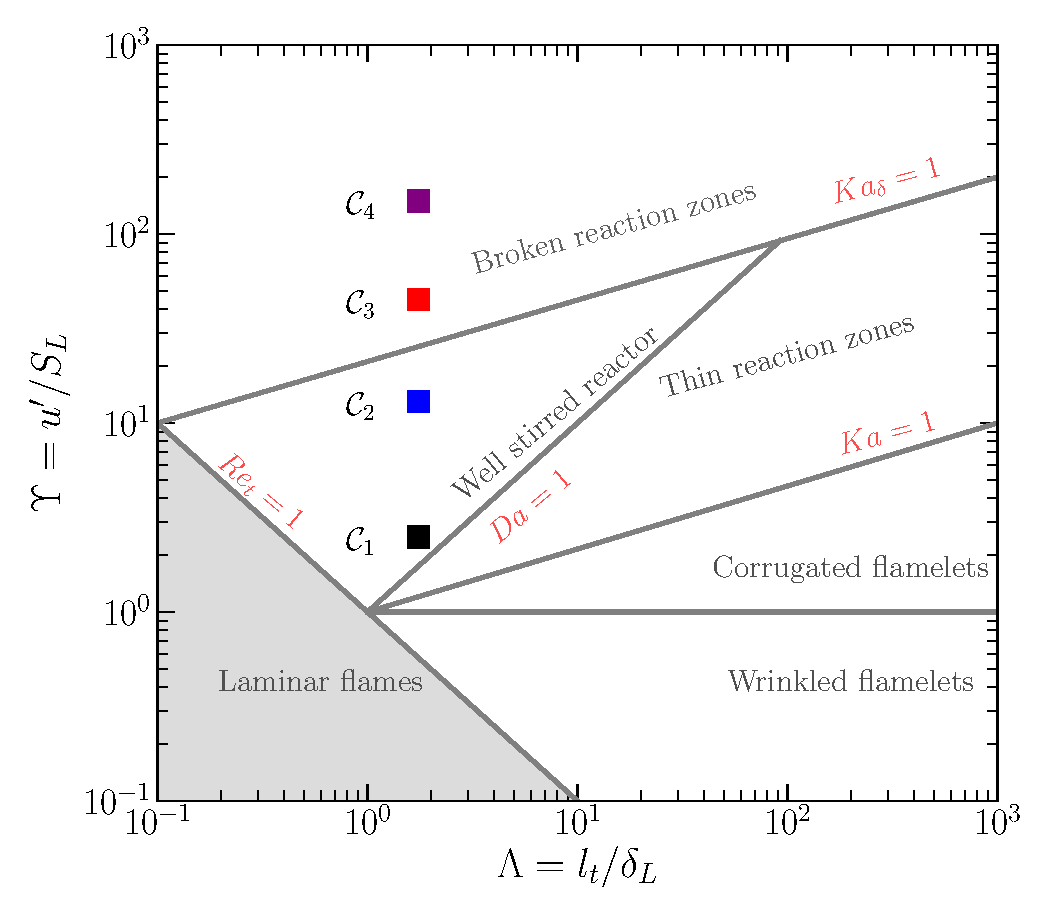
\includegraphics[width=0.7\textwidth]{./figs/borghi.pdf}
    \caption{Borghi combustion diagram showing the location of the cases $\mathcal{C}_1--\mathcal{C}_4$.
    Herein, Da and Ka are the Damk\"ohler and Karlovitz numbers, Re is the Reynolds number which is
    equal to (Da Ka)$^2$, and $Ka_\delta$ is the Karlovitz number based on the reaction zone thickness
    and approximated as $Ka_\delta\sim \mathrm{Ka}/100$.}
    \label{fig:borghi}
\end{figure}


\begin{table}[]
\centering
\begin{tabular}{ccrcrr}
\toprule
Case & $N$ & $\Upsilon$ & $Da$ & $Ka$ & $Re_t$ \\
\midrule
$\mathcal{C}_1$ & 128 & 2.5 & 0.700 & 3.0 & 32.5 \\
$\mathcal{C}_2$ & 128 & 13 & 0.135 & 35 & 169 \\
$\mathcal{C}_3$ & 256 & 45 & 0.039 & 228 & 584.5 \\
$\mathcal{C}_4$ & 512 & 150 & 0.012 & 1389 & 1948.4\\
\bottomrule
\end{tabular}
\caption{Grid resolution and initial turbulent-to-laminar flame speed ratio $\Upsilon \equiv u^{\prime}/S_L$,  Damk\"ohler, Da$=\Lambda/\Upsilon$, Karlovitz Ka$=(\Upsilon^3/\Lambda)^{1/2}$ and
 turbulent Reynolds number $\mathrm{Re}_t=u^{\prime}l_t/\nu$ used in the current DNS database.}
\label{tab:dns_details}
\end{table}

%=============================================================
Turbulence-flame interactions are often quantitatively investigated by means of characterizing
the two-way coupling between the turbulent flow field and the gradient of reactive scalar $\mathcal{Y}$.
%
This scalar can either be the mass fraction of a species present in the mixture, or the progress
variable which is a normalized quantity taking the values 0 and 1 in the fresh gases and the
burnt gases respectively.
%
The progress variable can be defined as the combination of a subset of species or in terms of the
temperature.
%
The evolution of the scalar $\mathcal{Y}$, which is considered as a progress variable in the following, 
is governed by the following transport equation
%
\begin{equation}
\frac{D\mathcal{Y}}{Dt} = \frac{1}{\rho} \nabla \cdot \left(\rho \mathcal{D}_{\mathcal{Y}}
\nabla \mathcal{Y}\right) +\dot{\omega}_{\mathcal{Y}}
\label{eq:trans_scalar}
\end{equation}
%
where $\mathcal{D}_{\mathcal{Y}}$ and $\dot{\omega}_{\mathcal{Y}}$ denote respectively the scalar's 
molecular diffusivity and the chemical reaction rate.
%
As the premixed flame evolves in the presence of turbulent fluctuations, the instantaneous flame 
front is subject to wrinkling which can be quantified using the variations and orientations of 
the flame normals pointing towards fresh gases and defined as :
\begin{equation}
\mathbf{n} = -\frac{\nabla \mathcal{Y}}{ \|\nabla \mathcal{Y}\|}
\end{equation}
%
where $\|\nabla \mathcal{Y}\| = \left[\mathcal{Y}^T\cdot\mathcal{Y}\right]^{1/2}$ is the scalar 
gradient magnitude, which can be used as a measure of the inverse of the local flame width $\delta_t$.
%
The dynamics of the scalar gradient magnitude, the local flame width and the normals to the 
iso-scalar surfaces are characterized with the equations

\begin{align}
\frac{D(\|\nabla \mathcal{Y}\|)}{Dt} &= - \mathbf{n} \cdot \frac{D(\nabla \mathcal{Y})}{Dt}
\label{eq:trans_magn_grad_c}\\
%
\frac{D(\|\nabla \mathcal{Y}\|^{-1})}{Dt} &= \|\nabla \mathcal{Y}\|^{-2 }\mathbf{n} \cdot 
\frac{D(\nabla \mathcal{Y})}{Dt}
\label{eq:trans_thickness}\\
%
\frac{D\mathbf{n}}{Dt} &= - \|\nabla \mathcal{Y}\|^{-1} (\mathcal{\boldsymbol{I}} - \mathbf{n}\mathbf{n}^T) \frac{D(\nabla \mathcal{Y})}{Dt}
\label{eq:trans_normals}
\end{align}
%
The equations \eqref{eq:trans_magn_grad_c}, \eqref{eq:trans_thickness} and  \eqref{eq:trans_normals}
depend on the transport equation of the scalar gradient, $\nabla \mathcal{Y}$, which is obtained
from \eqref{eq:trans_scalar} as 
%
\begin{equation}
\frac{D(\nabla \mathcal{Y})}{Dt} = \nabla \left( \frac{D\mathcal{Y}}{Dt}\right) + 
\|\nabla \mathcal{Y}\| \nabla \mathbf{u} \cdot\mathbf{n}
\label{eq:trans_scalar_grad_form0}
\end{equation}
%
This equation is often rewritten, by splitting the velocity gradient tensor into tensors of strain-rate, 
$\boldsymbol{\mathcal{S}}  = \frac{1}{2}\left(\nabla \mathbf{u} + \nabla \mathbf{u}^{T}\right)$, and rotation-rate, $\boldsymbol{\Omega}  = \frac{1}{2}\left(\nabla \mathbf{u} - \nabla \mathbf{u}^{T}\right)$, according to the Hermitian/skew-Hermitian Cauchy-Stokes decomposition as
%
\begin{dmath}
\frac{D(\nabla \mathcal{Y})}{Dt} = \nabla \left( \frac{D\mathcal{Y}}{Dt}\right) +
                   \|\nabla \mathcal{Y}\| \left(
                        \boldsymbol{\mathcal{S}} \cdot \mathbf{n} + 
                        \boldsymbol{\Omega} \cdot \mathbf{n}
                        \right) \\
       = \nabla \left( \frac{D\mathcal{Y}}{Dt}\right) +
        \|\nabla \mathcal{Y}\| \left(
        \boldsymbol{\mathcal{S}} \cdot \mathbf{n}
        +\frac{1}{2} \mathbf{n} \times \boldsymbol{\omega}
        \right)
\label{eq:cauchy_stokes}
\end{dmath}
%
where $\boldsymbol{\omega} = \nabla \times \mathbf{u}$ denotes the vorticity vector.
%
This form was widely used in prior studies, see for instance \cite{hamlington2011interactions,wacks2016flow,zhao2018dynamics}, to scrutinize the interactions of the small-scale turbulence, characterized by $\boldsymbol{\mathcal{S}}$ and $\boldsymbol{\omega}$, and the flame front.
%
Indeed, as highlighted by the equations above, the terms perpendicular (parallel) to the flame
normals, are expected to directly influence the dynamics of the normals (local width).
%
Consequently, both the strain-rate and the vorticity terms in the equation \eqref{eq:cauchy_stokes}
play a role in the dynamics of the flame wrinkling and orientation, whereas only the strain-rate
term affects $\delta_t$.
%
In light of the above, the turbulence-flame interactions are reflected by the alignments of flame 
normals with the normalized vorticity vector $\hat{\boldsymbol{\omega}} = \boldsymbol{\omega}/\|\boldsymbol{\omega}\|$ and with the principal directions $\mathbf{e}_i$ of the strain-rate tensor $\boldsymbol{\mathcal{S}}$.
%
The alignments are given with the absolute value of the cosine of the angle between two vectors,
such as the value 1 indicates a perfect alignment and 0 refer to a perfect misalignment 
(perpendicularity).
%
Given the symmetry of the strain-rate tensor, the eigenvalues $\mathbf{e}_i$, correspond to the
three real eigenvalues, $\lambda_i$, of $\boldsymbol{\mathcal{S}}$ ordered as $
\lambda_1>\lambda_2>\lambda_3$, where $\mathbf{e}_1$, $\mathbf{e}_2$ and $\mathbf{e}_3$ can be 
referred to as the extensive, intermediate and compressive directions.
%
One of the key findings of this family of analysis, conducted either on the passive and reactive 
scalars with passive chemical reactions or flame characterized with a high Karlovitz number,  
is preferential alignment of the scalar gradient with the most compressive direction 
$\mathbf{e}_3$ \cite{ashurst1987alignment,rutland1993direct,kim2007scalar,chakraborty2007influence,hamlington2011interactions,hartung2008effect,swaminathan2006interaction}.
%
However, this behaviour is altered in weak to moderate turbulence (low Karlovitz) where the 
flame-induced thermal expansion affects the turbulence-scalar interaction and the normals are
aligned with the most extensive direction $\mathbf{e}_1$ \cite{chakraborty2007influence,
cifuentes2014local,chakraborty2007comparison}.\\


Obviously, as demonstrated above, the classical decomposition of the velocity tensor has led
to important conclusions in terms of turbulence-flame interactions.
%
However, this decomposition obscures the understanding of some of the processes taking place in the
interaction of the flame with the turbulent flow field.
%
Indeed, as highlighted by a certain number of recent studies \cite{kolavr2007vortex,gao2019rortex,nagata2020triple}, the Hermitian/skew-Hermitian decomposition is constrained by its inability
to segregate pure local normal-straining and rigid-body-rotation effects from non--local dynamics
induced by shearing, as the latter is an intrinsic part of both strain-rate and vorticity tenors.
%
More recently, by performing a complex Schur decomposition of $\nabla \mathbf{u}$,
\citet{keylock2018schur}, dissociated the shear contribution from the other dynamics of the 
velocity gradient.
%
In this framework, the decomposition introduced by \citet{keylock2018schur}, isolates the local
dynamics, which are associated to the eigenvalues, from the non-local effects induced by the vortical
structures following
%
\begin{equation}
\boldsymbol{\mathcal{P}}^* \nabla \mathbf{u} \boldsymbol{\mathcal{P}} =  \mathcal{T} 
            = \boldsymbol{\mathcal{D}_{\lambda}}  +  \boldsymbol{\mathcal{N}}
\label{eq:complex_schur}
\end{equation} 
%
where $(.)^*$ is the Hermitian operator, $\boldsymbol{\mathcal{P}} \in \mathbb{C}^{(3\times3)}$ is a unitary
matrix, \ie $\boldsymbol{\mathcal{P}\mathcal{P}}^*=\mathbf{I}$ and $\boldsymbol{\mathcal{T}} \in \mathbb{C}^{(3\times3)}$ is an upper-triangular matrix.
%
The matrix $\boldsymbol{\mathcal{D}_{\lambda}}$ is the diagonal matrix composed of $\nabla \mathbf{u}$ eigenvalues and $\boldsymbol{\mathcal{N}}$ is a strictly upper-triangular matrix such that
%
\begin{equation}
\boldsymbol{\mathcal{D}_{\lambda}} =   
\begin{pmatrix}
\lambda_1 & 0 & 0\\ 
0         & \lambda_2    & 0\\
0         & 0            & \lambda_3
\end{pmatrix}
%
~~~~~~,~~~~~
\boldsymbol{\mathcal{N}} = \begin{pmatrix}
0 & \gamma_{12} & \gamma_{13}\\ 
0         & 0    & \gamma_{23}\\
0         & 0            & 0
\end{pmatrix}
\end{equation}
where $\lambda_i$ refer to the eigenvalues of the velocity gradient tensor ordered in the 
increasing order of their norms.


The approach based on the equation \eqref{eq:complex_schur} presents the advantage of projecting the
non-normal (non-local) effects into an upper-triangular matrix that can be treated in an analogous
manner to the analysis based on principal eigenvectors, which eases the interpretation of the
respective effects of normal and non--normal contributions.
%
as a matter of fact, the concept embodied by the equation \eqref{eq:complex_schur} has proven to be 
an effective tool to provide concrete explanations concerning the alignments properties, such
as the one between the vorticity vector and the intermediate strain eigenvector and demonstrates
the key role played by non-normality \cite{keylock2018schur}.


The present work aims at reinterpreting some of the classical results obtained in 
the context of turbulence-flame interaction, in the light of concept presented above, and seeking
a deeper insight and further clarity into the phenomena taking place in a such interaction.
%
In view of this, the transport equation of the scalar gradient \eqref{eq:cauchy_stokes}
is re-expressed as:
%
\begin{equation}
\frac{D(\nabla \mathcal{Y})}{Dt} = \nabla \left( \frac{D\mathcal{Y}}{Dt}\right) +
        \|\nabla \mathcal{Y}\| \left(
        \boldsymbol{\mathcal{A_L}} \cdot \mathbf{n}
        +\boldsymbol{\mathcal{A_N}} \cdot \mathbf{n}
        \right)
\label{eq:trans_grad_schur}
\end{equation}
%
where $\boldsymbol{\mathcal{A_L}} \equiv \boldsymbol{\mathcal{P}} \boldsymbol{\mathcal{D}_{\lambda}}
\boldsymbol{\mathcal{P}}^*$ and $\boldsymbol{\mathcal{A_N}} \equiv \boldsymbol{\mathcal{P}} \boldsymbol{\mathcal{N}} \boldsymbol{\mathcal{P}}^*$  denote respectively the local (normal) and non-local 
(non-normal) components of the velocity gradient.

As a starting point of the current analysis, the relative importance of the non-normal effects across
the whole flame brush is scrutinized.
%
In the present analysis, the flame is characterized by the progress variable based on the temperature, \ie
%
\begin{equation}
    c = \frac{T - T^u}{T^b-T^u}
\end{equation}
%
where $T(Y, \mathbf{x})$ is the mixture temperature and the superscripts $u$ and $b$ refer, 
respectively to the fresh reactants and the fully burnt gases states.
%
\autoref{fig:snapshots_prog_var} displays the three-dimensional iso-surfaces of $c$ for the four 
cases considered in the DNS database.
%
\begin{figure}[htpb]
\centering
\begin{subfigure}{.5\textwidth}
\centering

\includegraphics[width=.5\textwidth]{./figs/progvar/cmap.pdf}
\end{subfigure}

\vspace{2em}

\begin{subfigure}{.48\textwidth}
\centering
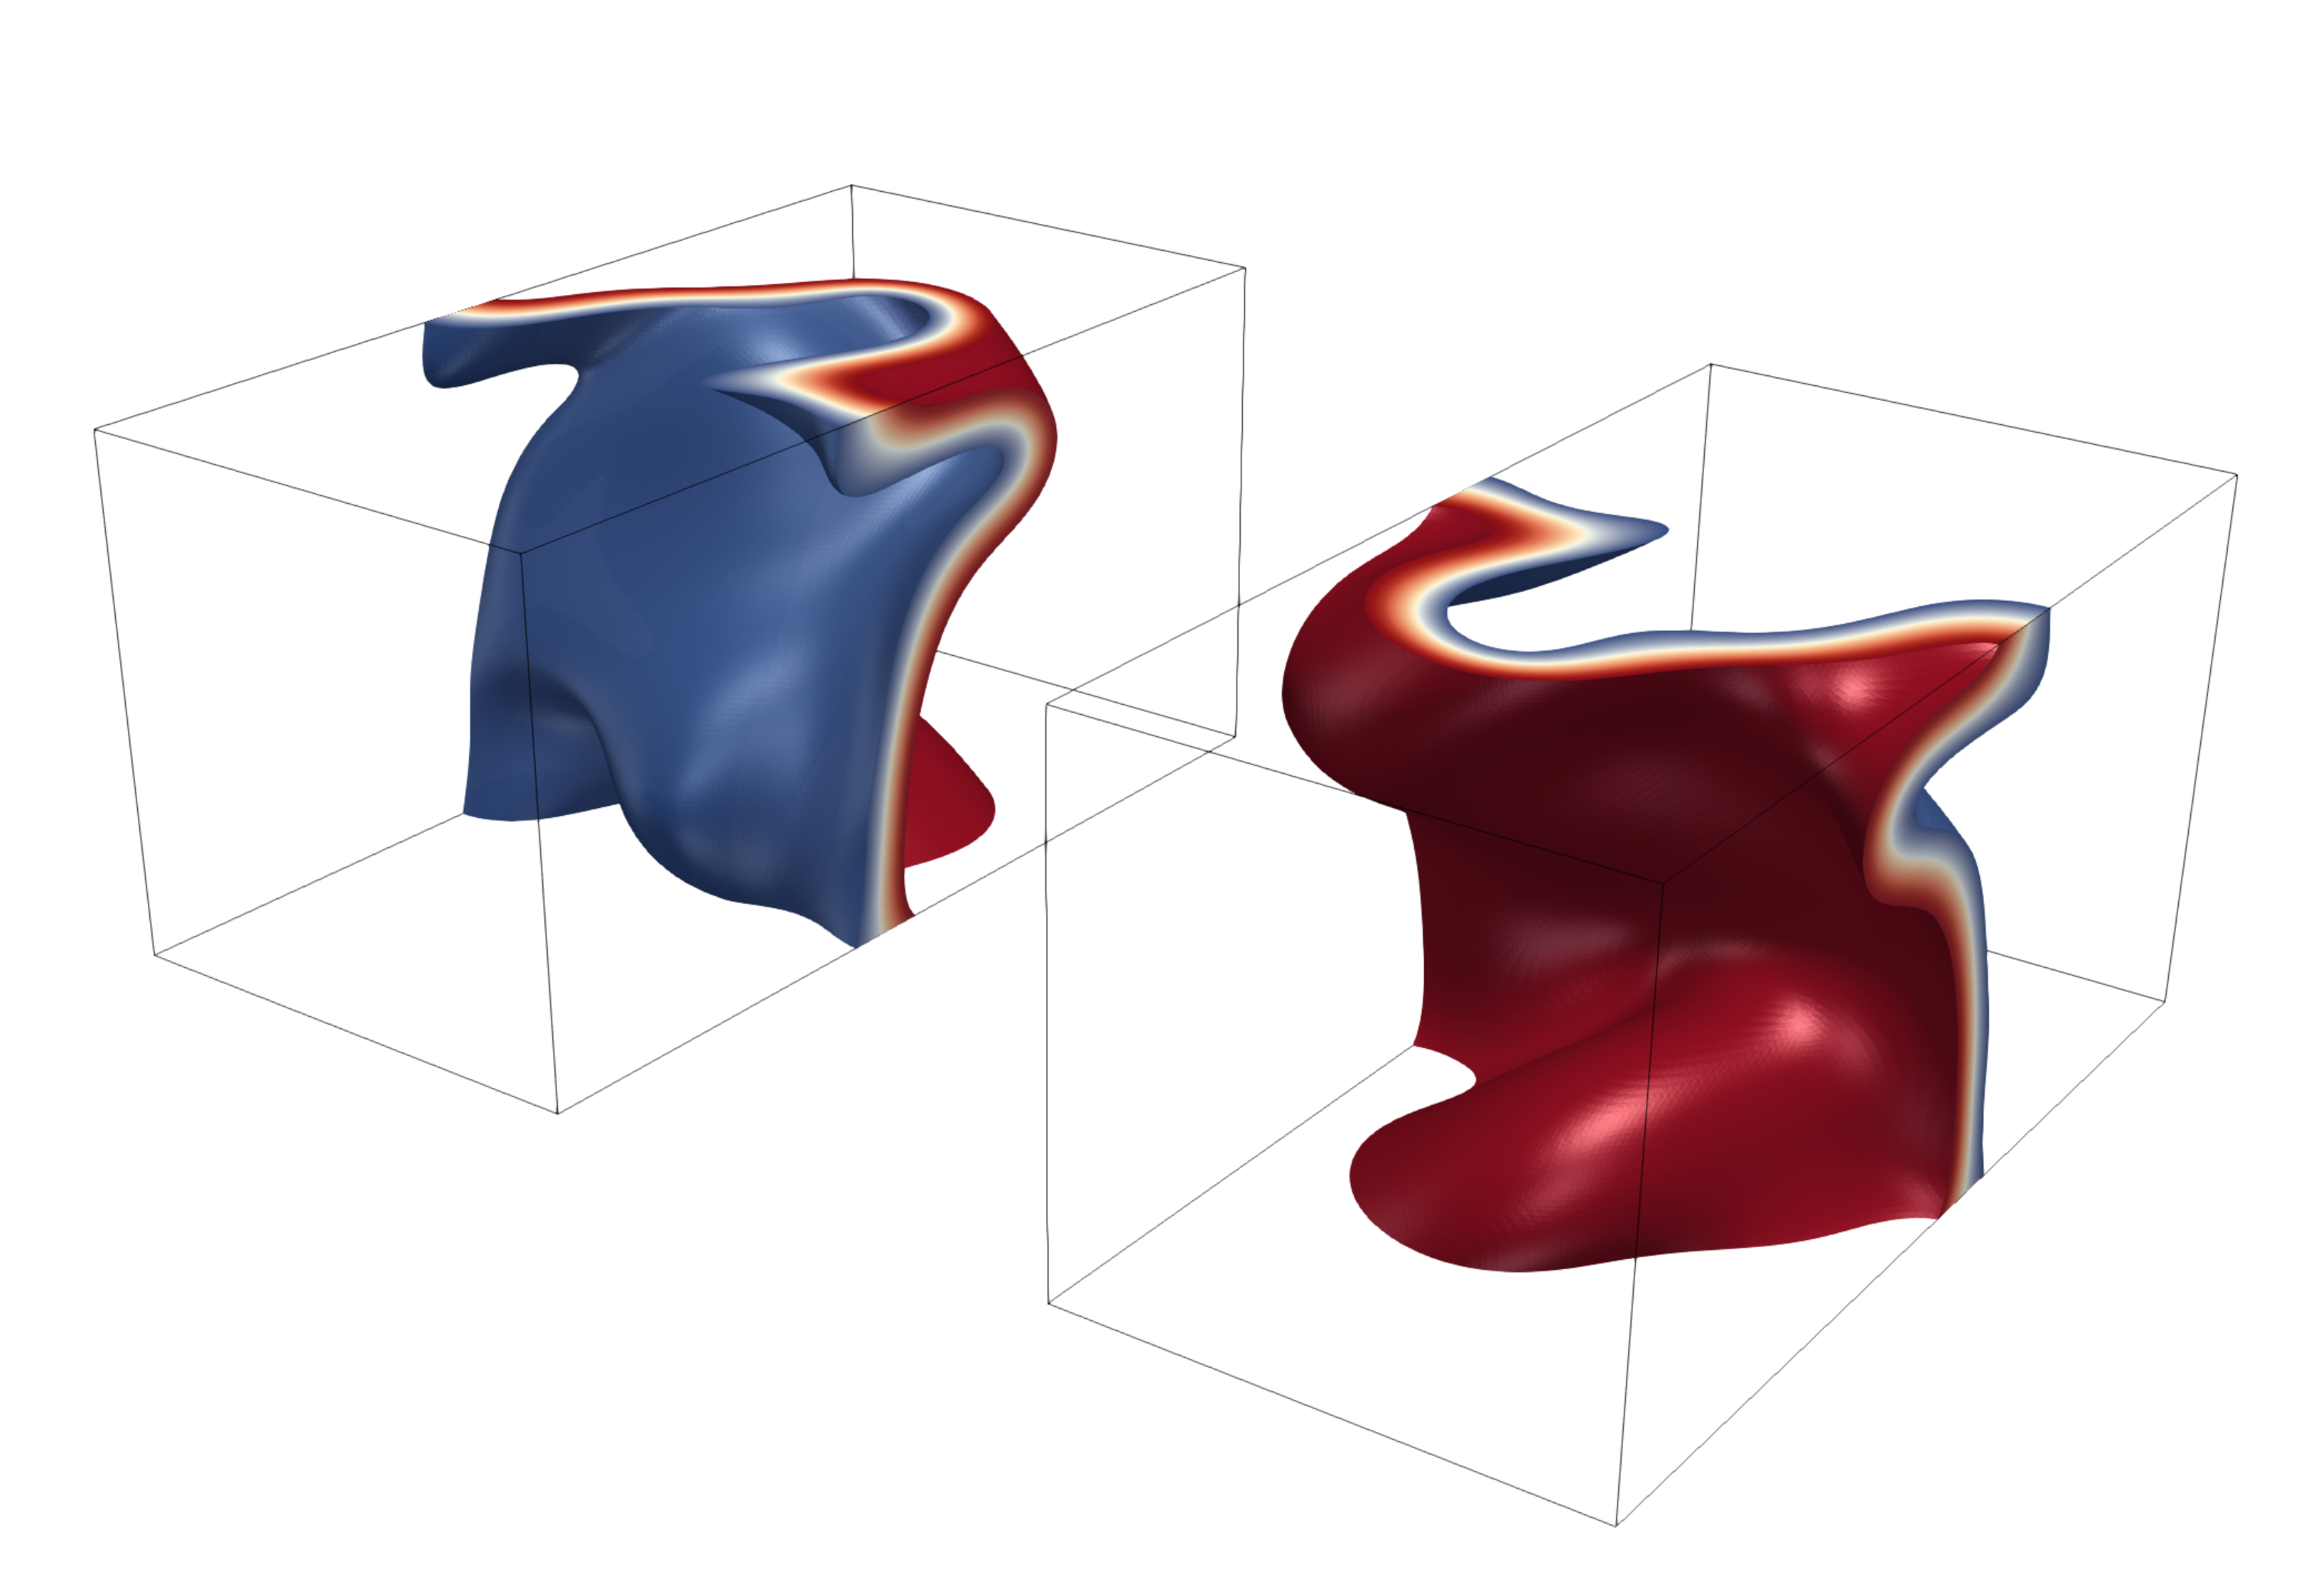
\includegraphics[width=.99\textwidth]{./figs/progvar/case1.pdf}
\caption{Case $\mathcal{C}_1$}
\label{fig:progvar_contour_case1}
\end{subfigure}
%
\begin{subfigure}{.48\textwidth}
\centering
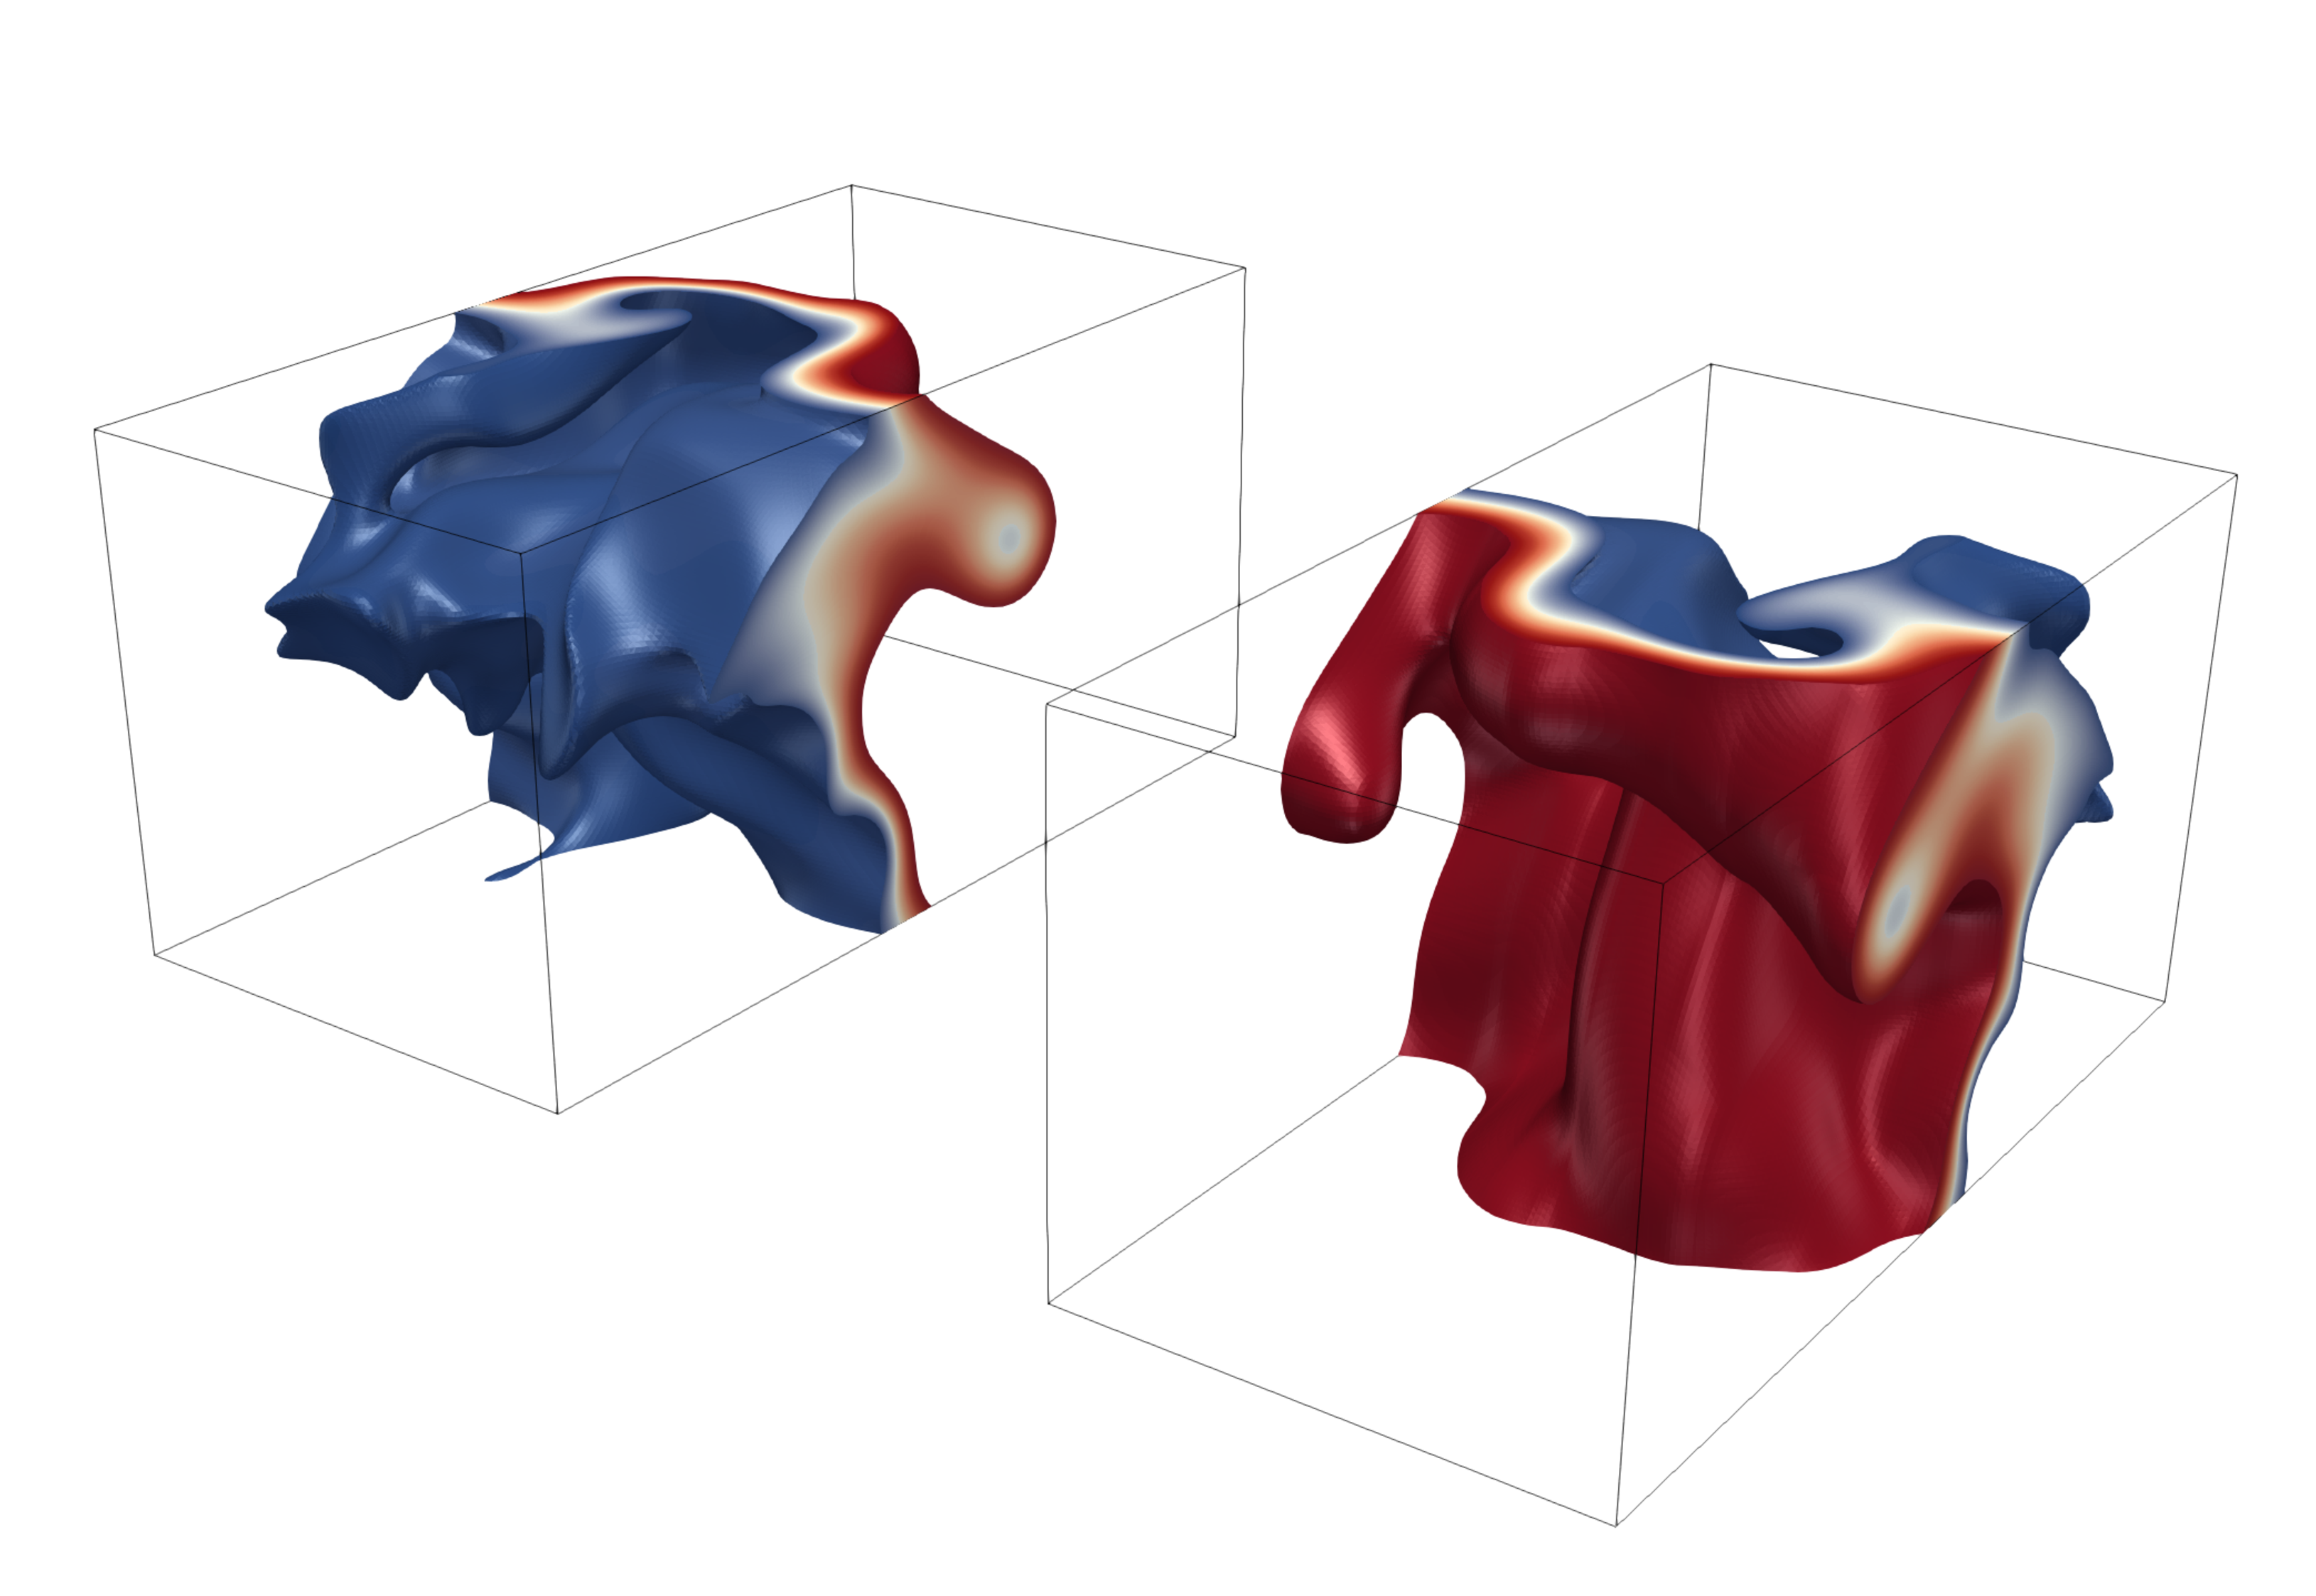
\includegraphics[width=.99\textwidth]{./figs/progvar/case2.pdf}
\caption{Case $\mathcal{C}_2$}
\label{fig:progvar_contour_case2}
\end{subfigure}

\begin{subfigure}{.48\textwidth}
\centering
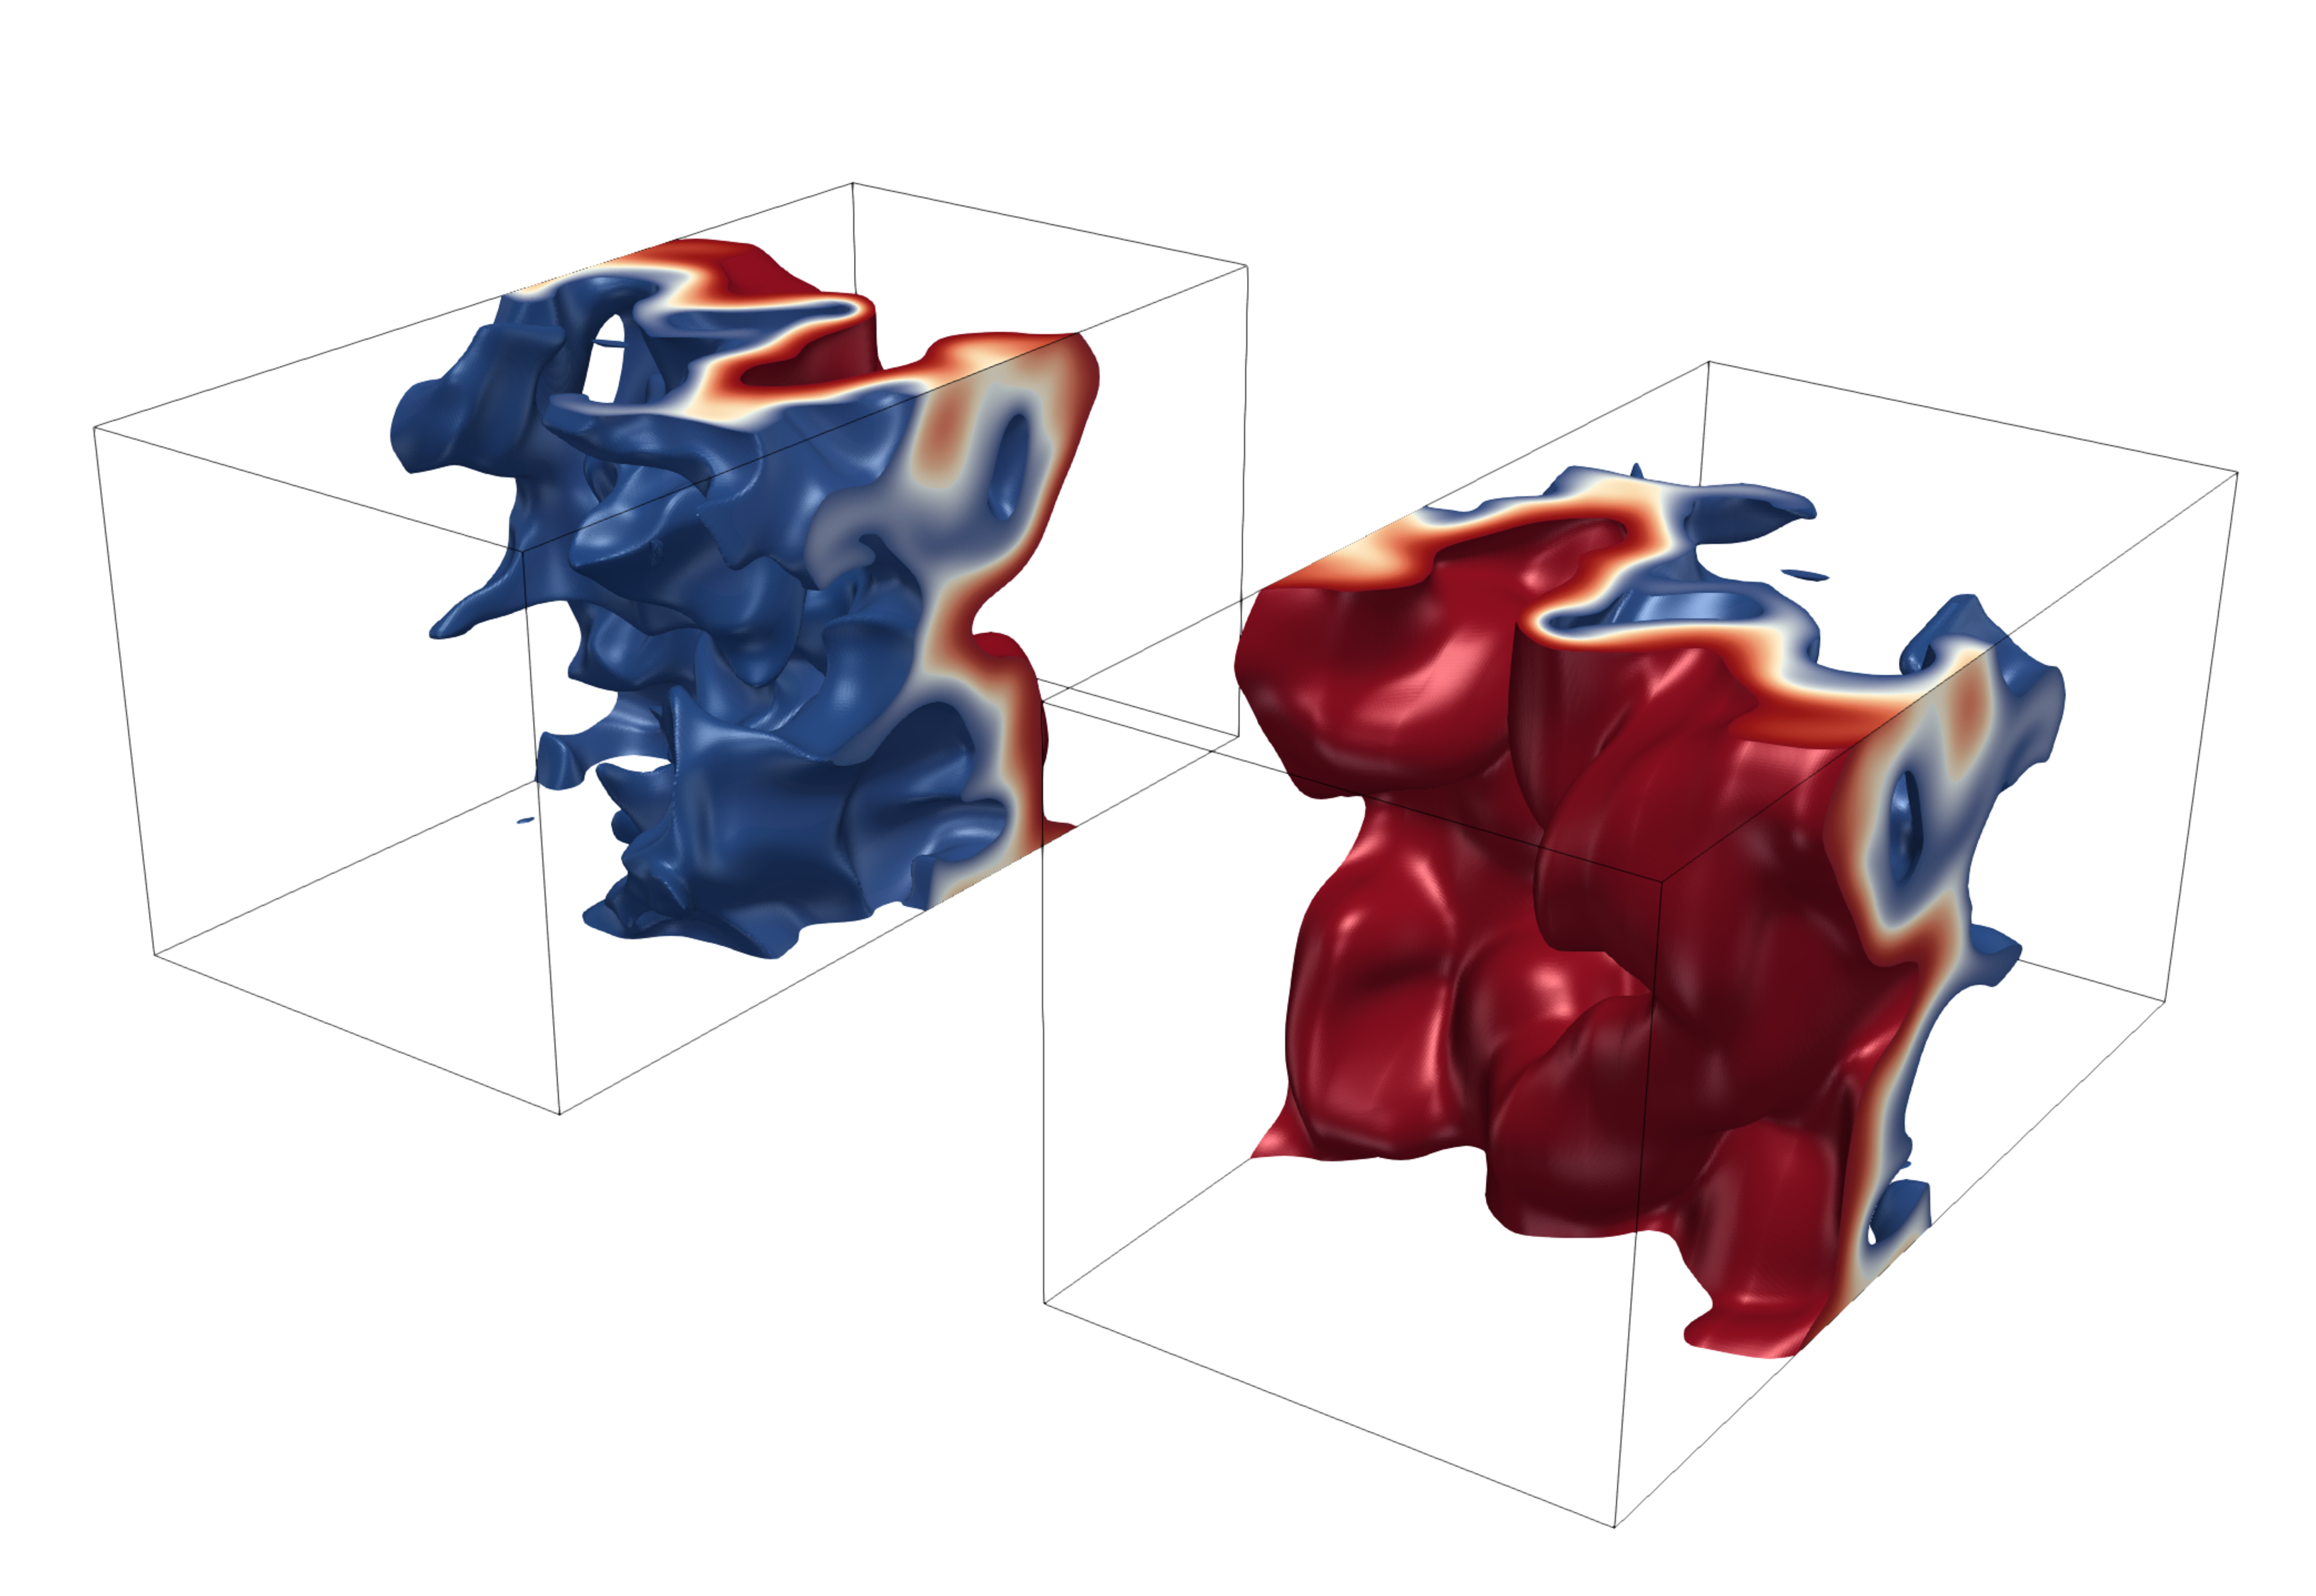
\includegraphics[width=.99\textwidth]{./figs/progvar/case3.pdf}
\caption{Case $\mathcal{C}_3$}
\label{fig:progvar_contour_case3}
\end{subfigure}
%
\begin{subfigure}{.48\textwidth}
\centering
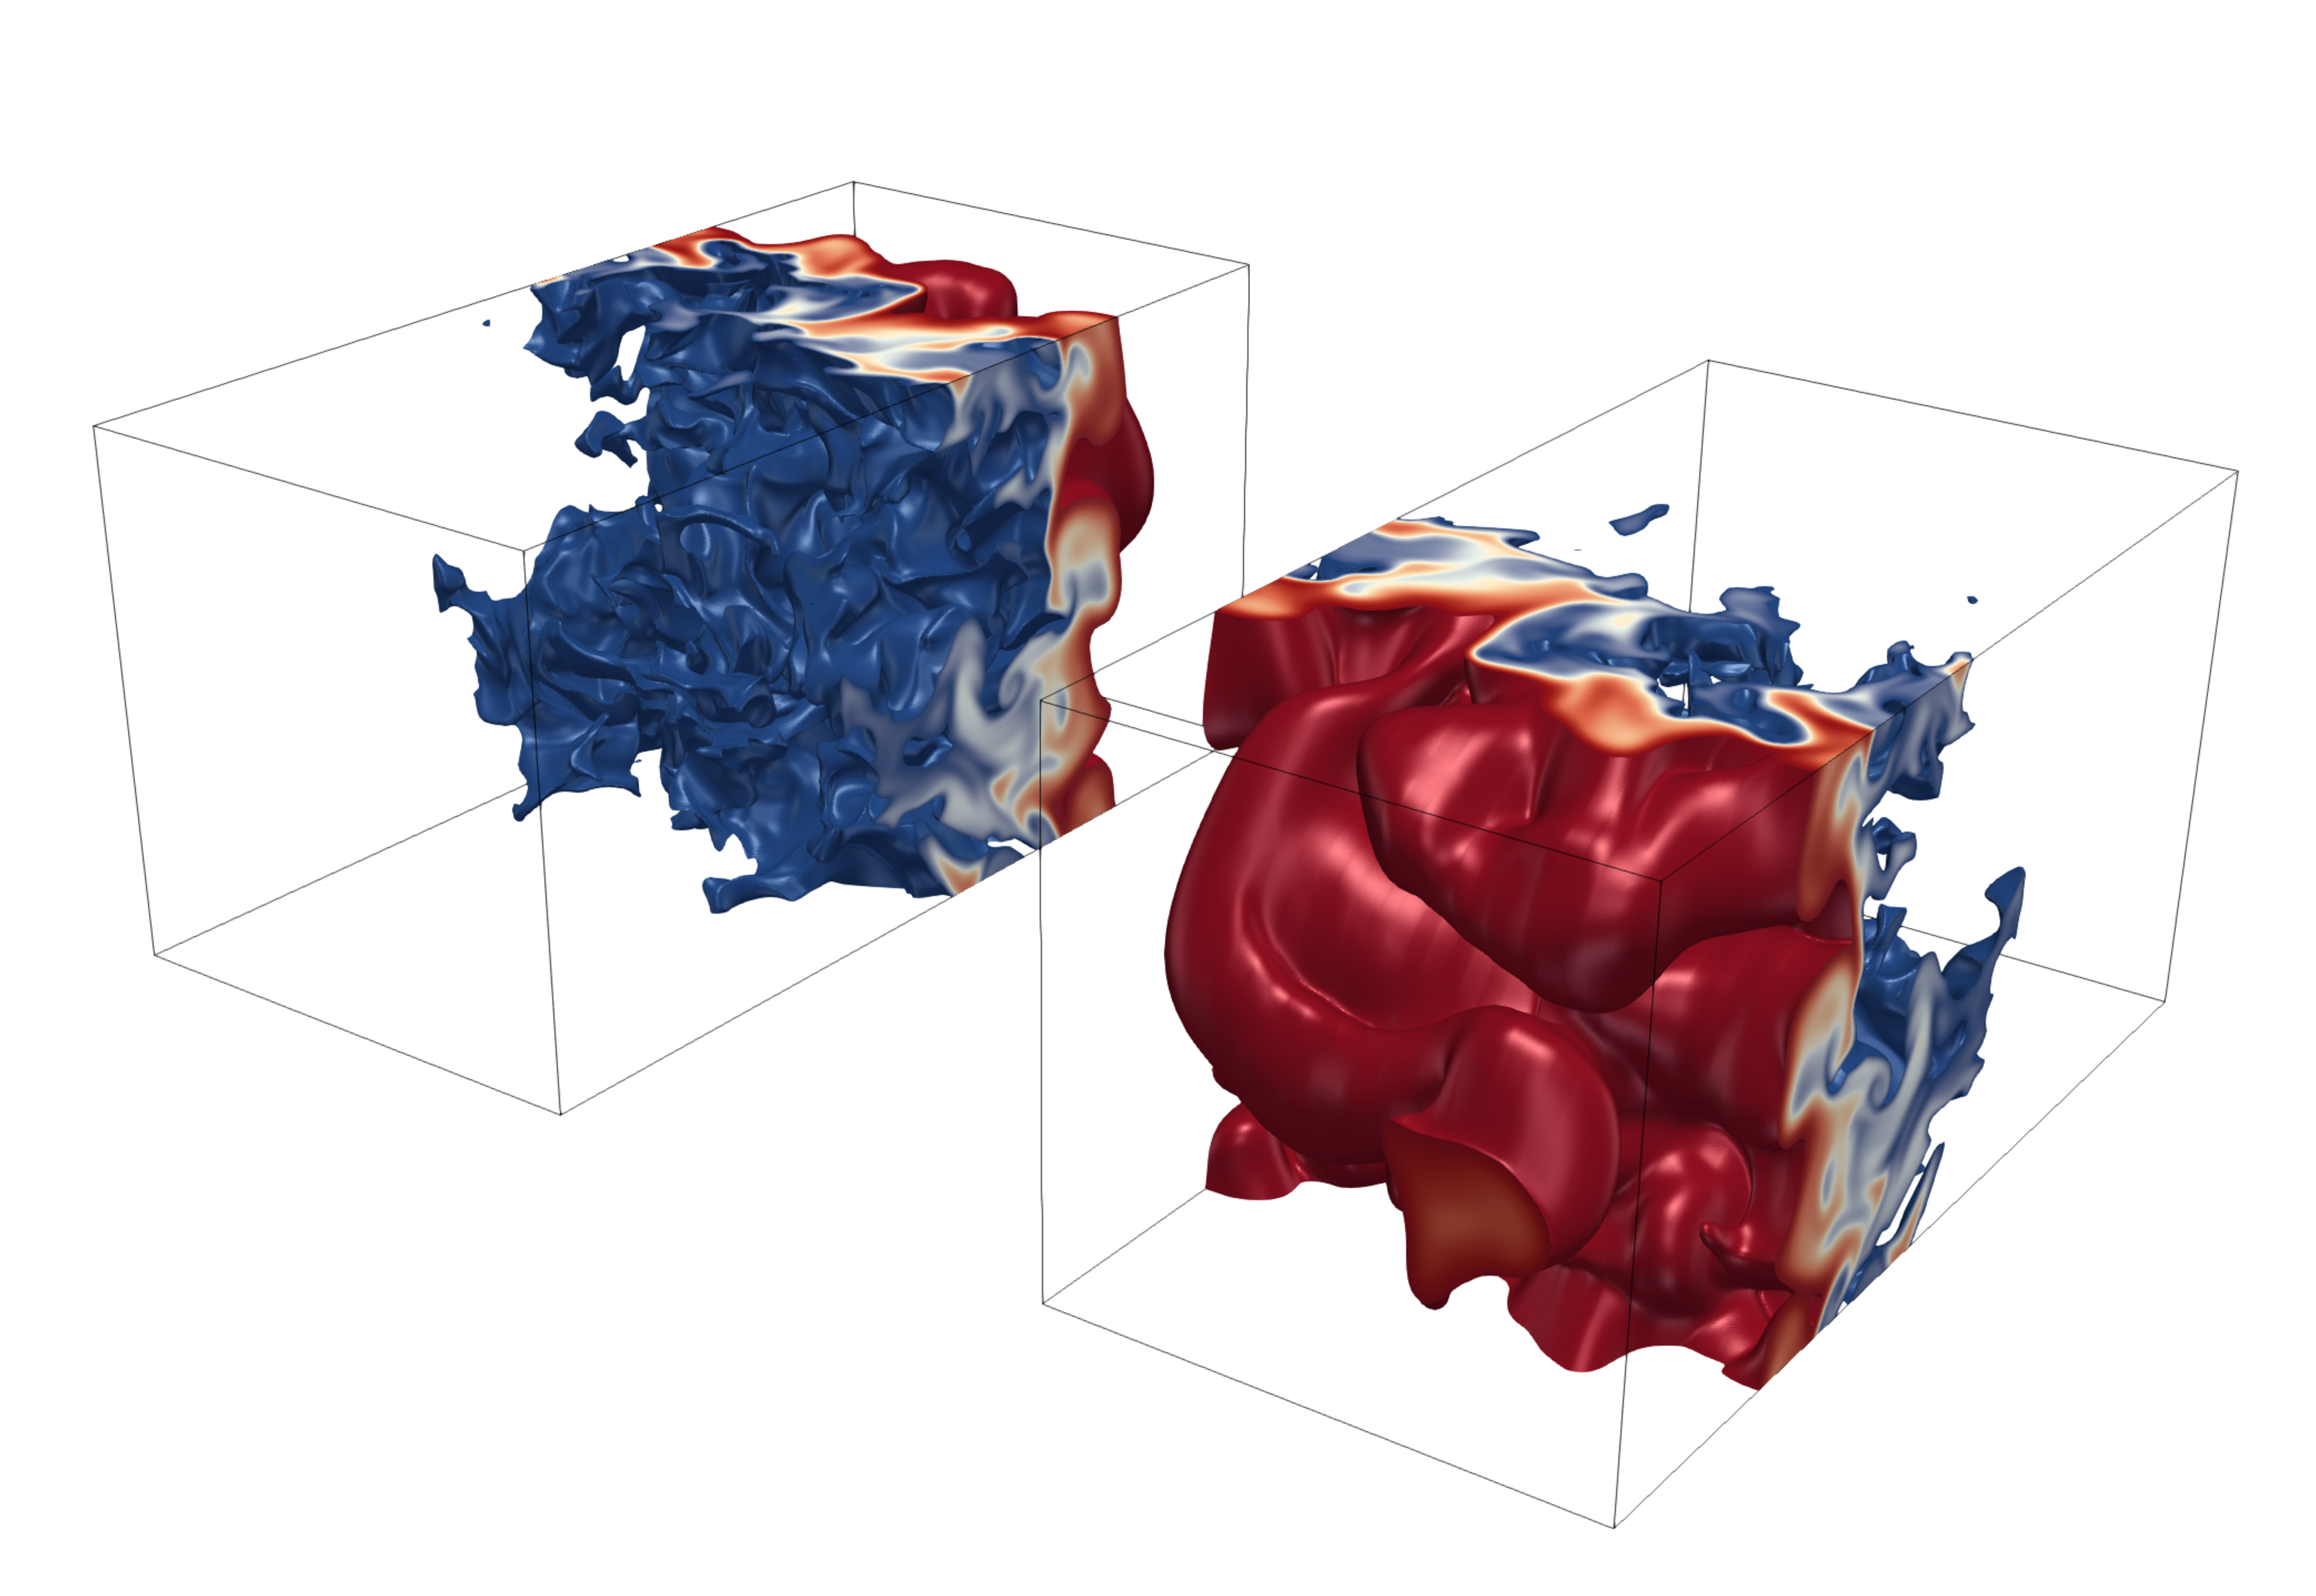
\includegraphics[width=.99\textwidth]{./figs/progvar/case4.pdf}
\caption{Case $\mathcal{C}_4$}
\label{fig:progvar_contour_case4}
\end{subfigure}
\caption{Instantaneous iso-surfaces of the progress variable based on the mixture temperature,
for (a) $\mathcal{C}_1$, (b) $\mathcal{C}_2$, (c) $\mathcal{C}_3$, and (d) $\mathcal{C}_4$.
%
The left column displays the fresh reactants side with the iso-surface $c^*=0.4$ and the right column
the burnt gases side with the iso-surface $c^*=0.9$.}
\label{fig:snapshots_prog_var}
\end{figure}
%
Since the dynamics of the velocity gradient are resulting from the superposition of the normal and 
non-normal contributions given by  $\|\mathcal{A}_{\mathcal{L}}\|$ and  $\|\mathcal{A}_{\mathcal{N}}\|$
respectively, where $\|\mathcal{M}\|$ refer to the Frobenius norm of the matrix $\mathcal{M}$, \ie
$\|\mathcal{M}\|^2 = \mathrm{tr}(\mathcal{M}\mathcal{M}^*)= \sum_{i, j=1}^3\mathrm{tr} |\mathcal{M}_{i,j}|^2$, the relative importance of normal/non-normal effects can be estimated on the basis of the following standardized difference
%
\begin{equation}
    \kappa_{\mathcal{A}_{\mathcal{L}}, \mathcal{A}_{\mathcal{N}}} = \frac{\|\mathcal{A}_{\mathcal{L}}\| -
    \|\mathcal{A}_{\mathcal{N}}\|}{\|\mathcal{A}_{\mathcal{L}}\|+\|\mathcal{A}_{\mathcal{N}}\|}
\end{equation}
%
By definition, $-1<\kappa_{\mathcal{A}_{\mathcal{L}}, \mathcal{A}_{\mathcal{N}}}<1$, where a value
of -1 indicates a dominance of non-normal effects, whereas $\kappa_{\mathcal{A}_{\mathcal{L}}, \mathcal{A}_{\mathcal{N}}}=1$ reflects a weak impact of non-normality and making it acceptable to approximate
the flow dynamics by the eigenvalues-based approach.
%
An instantaneous plot of this indicator is given by \autoref{fig:kappa_contour} which illustrates
visually the comparability of the non-normal contribution to the one associated to the eigenvalues 
part and thus the importance of the non-local effects across all the flame brush.%
%
\begin{figure}[htpb]
\centering
\begin{subfigure}{.48\textwidth}
\hspace{-5em}

\includegraphics[width=1.5\textwidth]{./figs/kappa/cmap.pdf}
\end{subfigure}

\vspace{2em}

\begin{subfigure}{.48\textwidth}
\centering
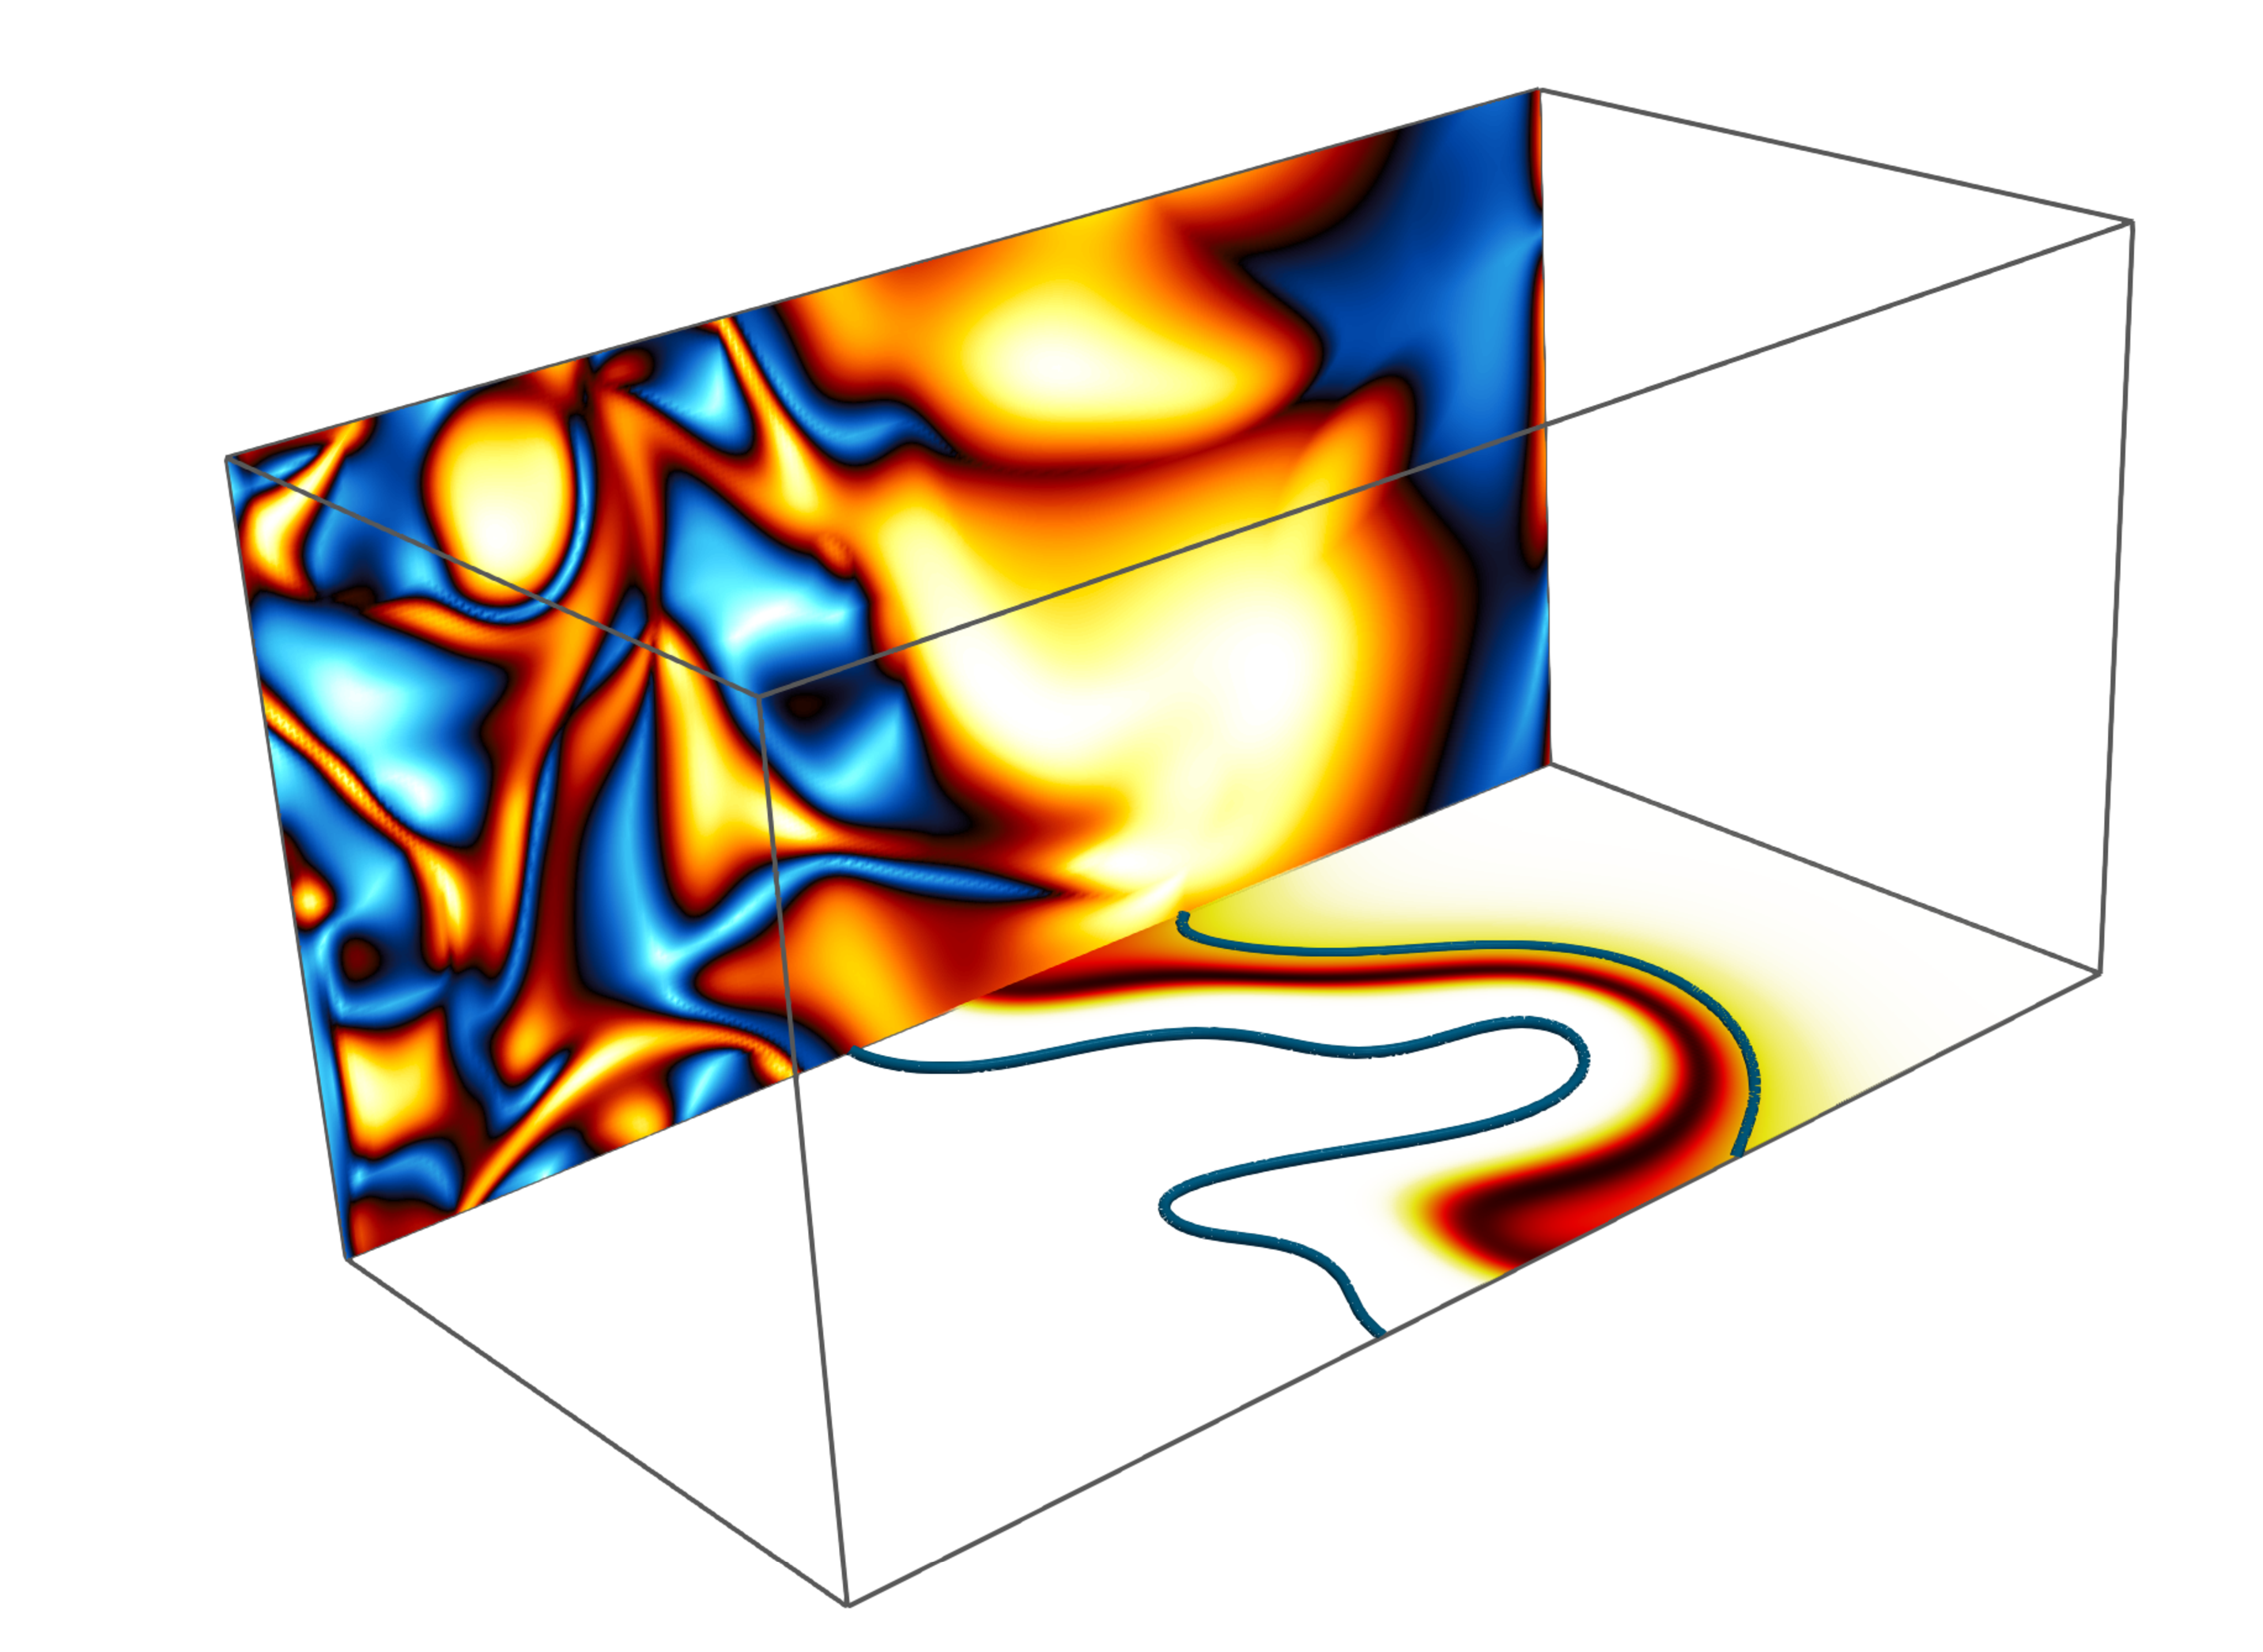
\includegraphics[width=.99\textwidth]{./figs/kappa/case1.pdf}
\caption{Case $\mathcal{C}_1$}
\label{fig:kappa_contour_case1}
\end{subfigure}
%
\begin{subfigure}{.48\textwidth}
\centering
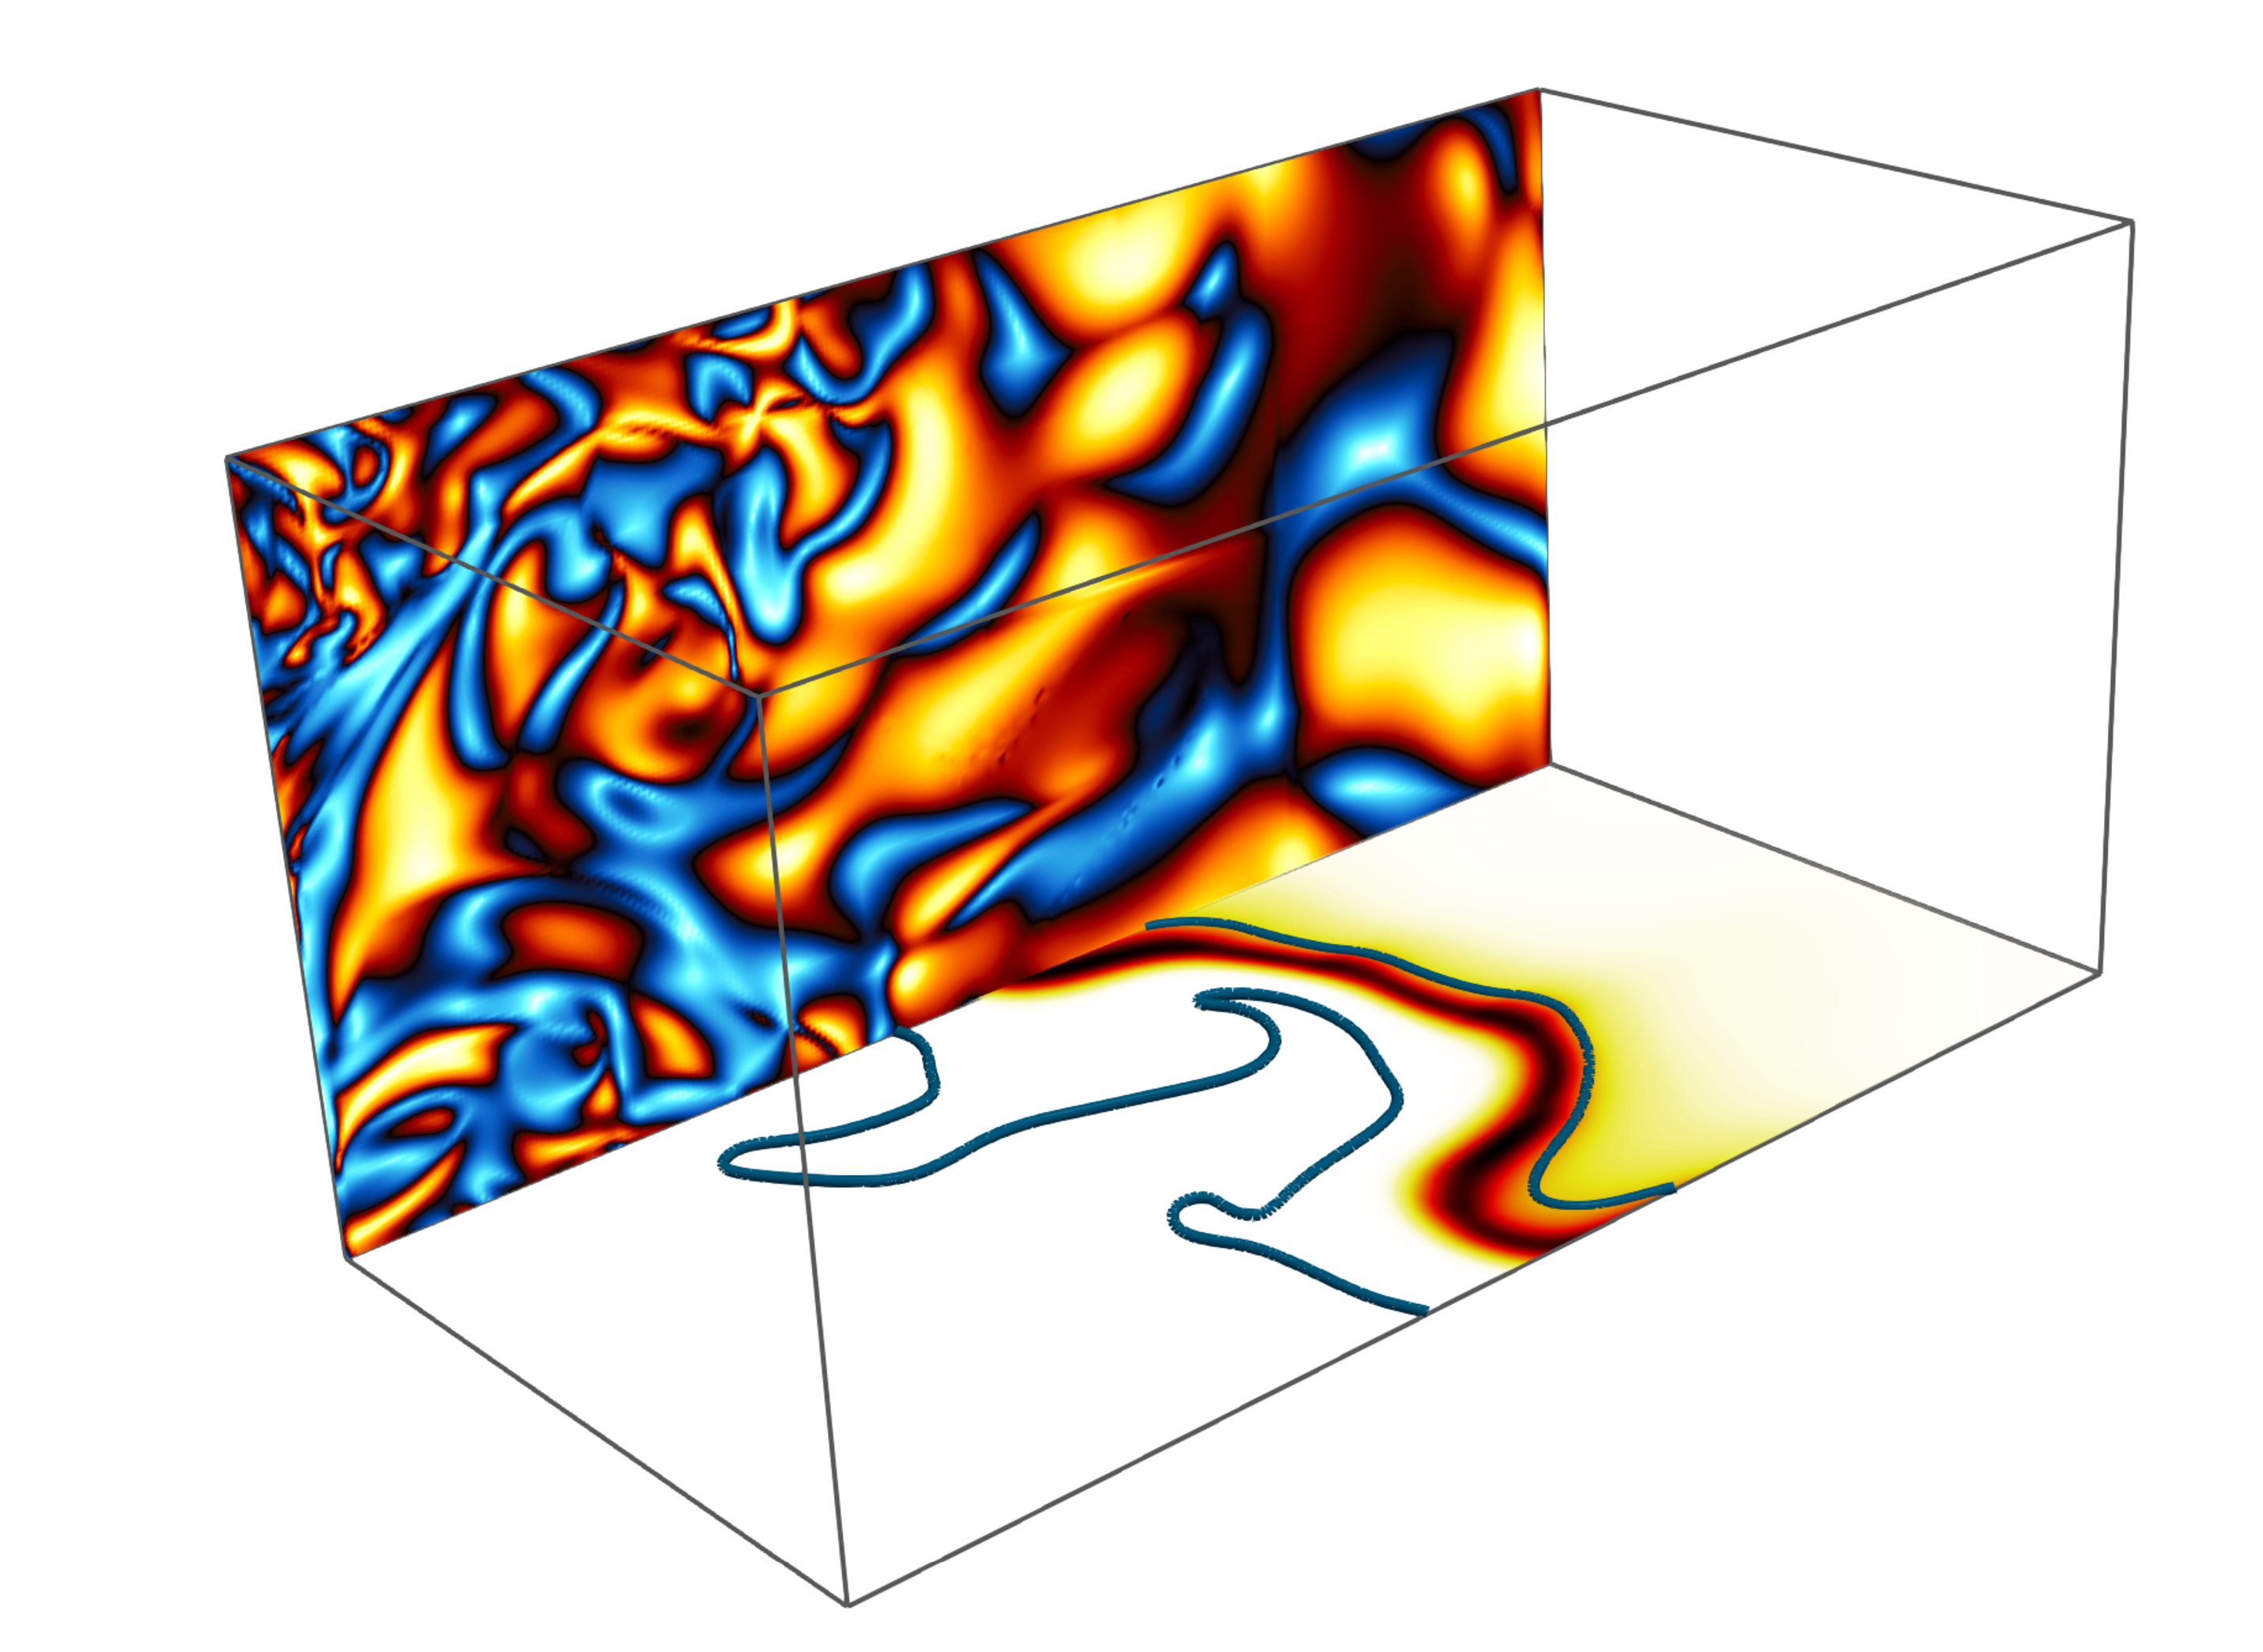
\includegraphics[width=.99\textwidth]{./figs/kappa/case2.pdf}
\caption{Case $\mathcal{C}_2$}
\label{fig:kappa_contour_case2}
\end{subfigure}

\begin{subfigure}{.48\textwidth}
\centering
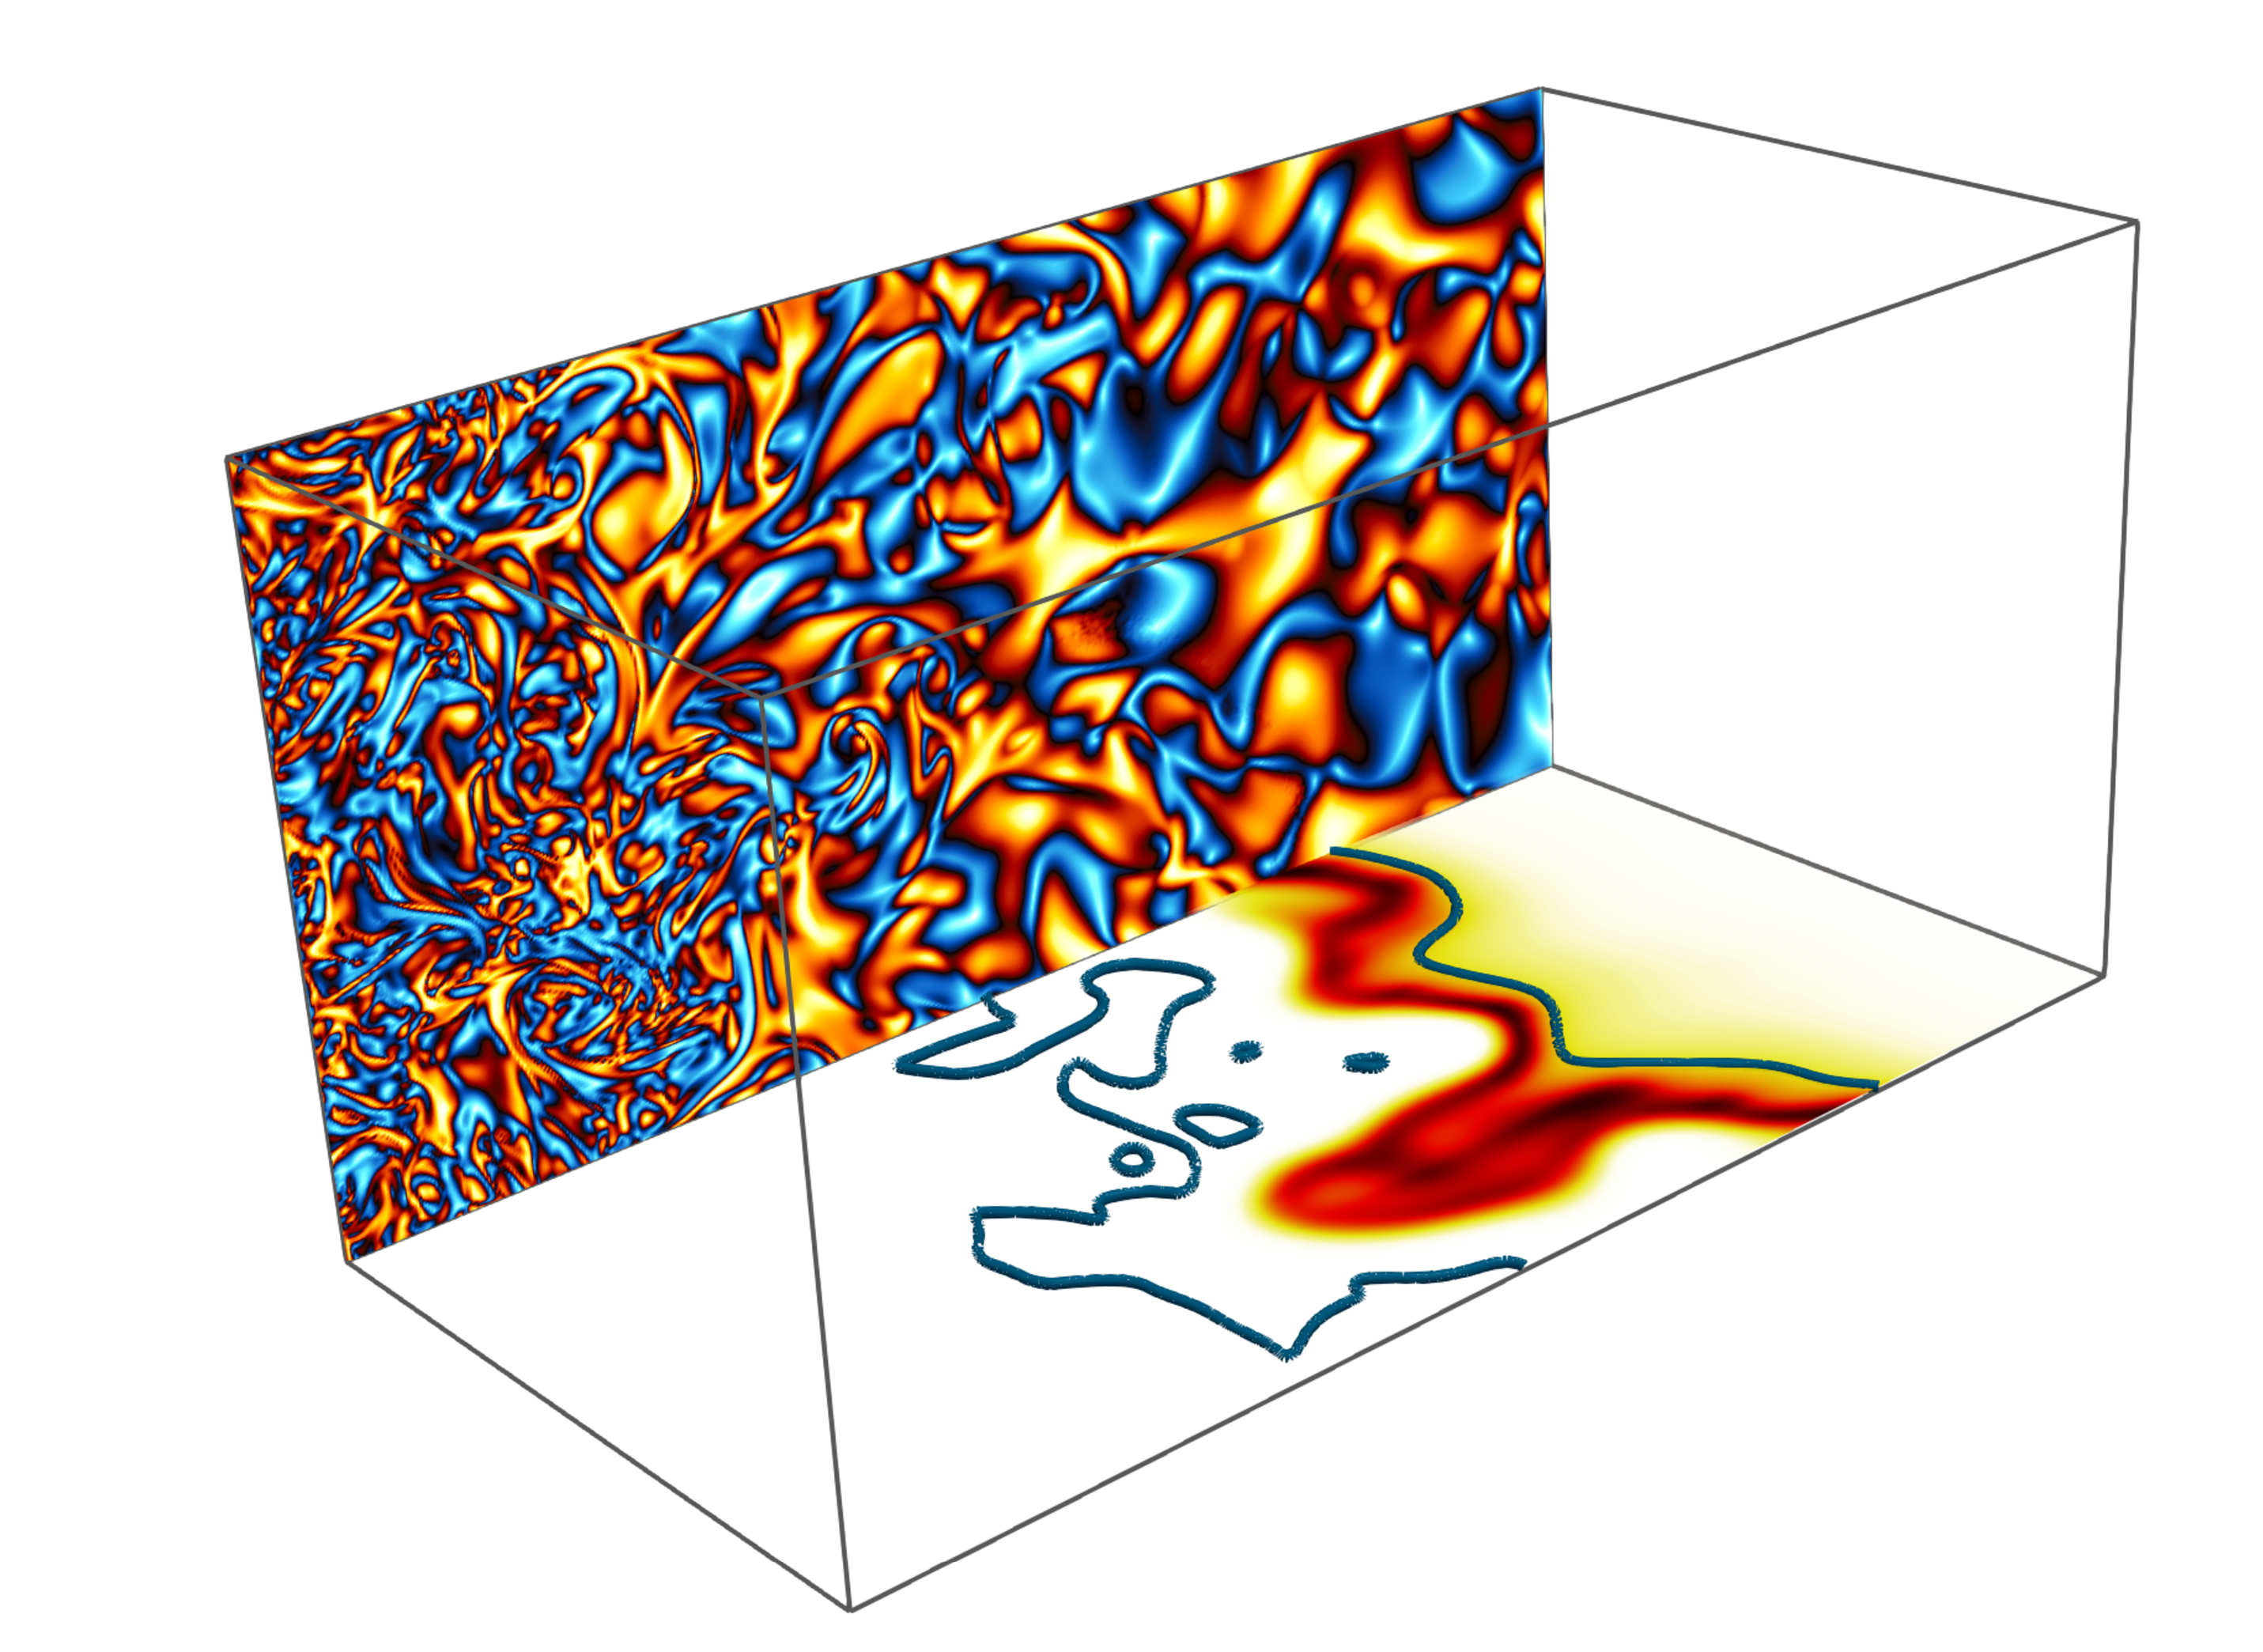
\includegraphics[width=.99\textwidth]{./figs/kappa/case3.pdf}
\caption{Case $\mathcal{C}_3$}
\label{fig:kappa_contour_case3}
\end{subfigure}
%
\begin{subfigure}{.48\textwidth}
\centering
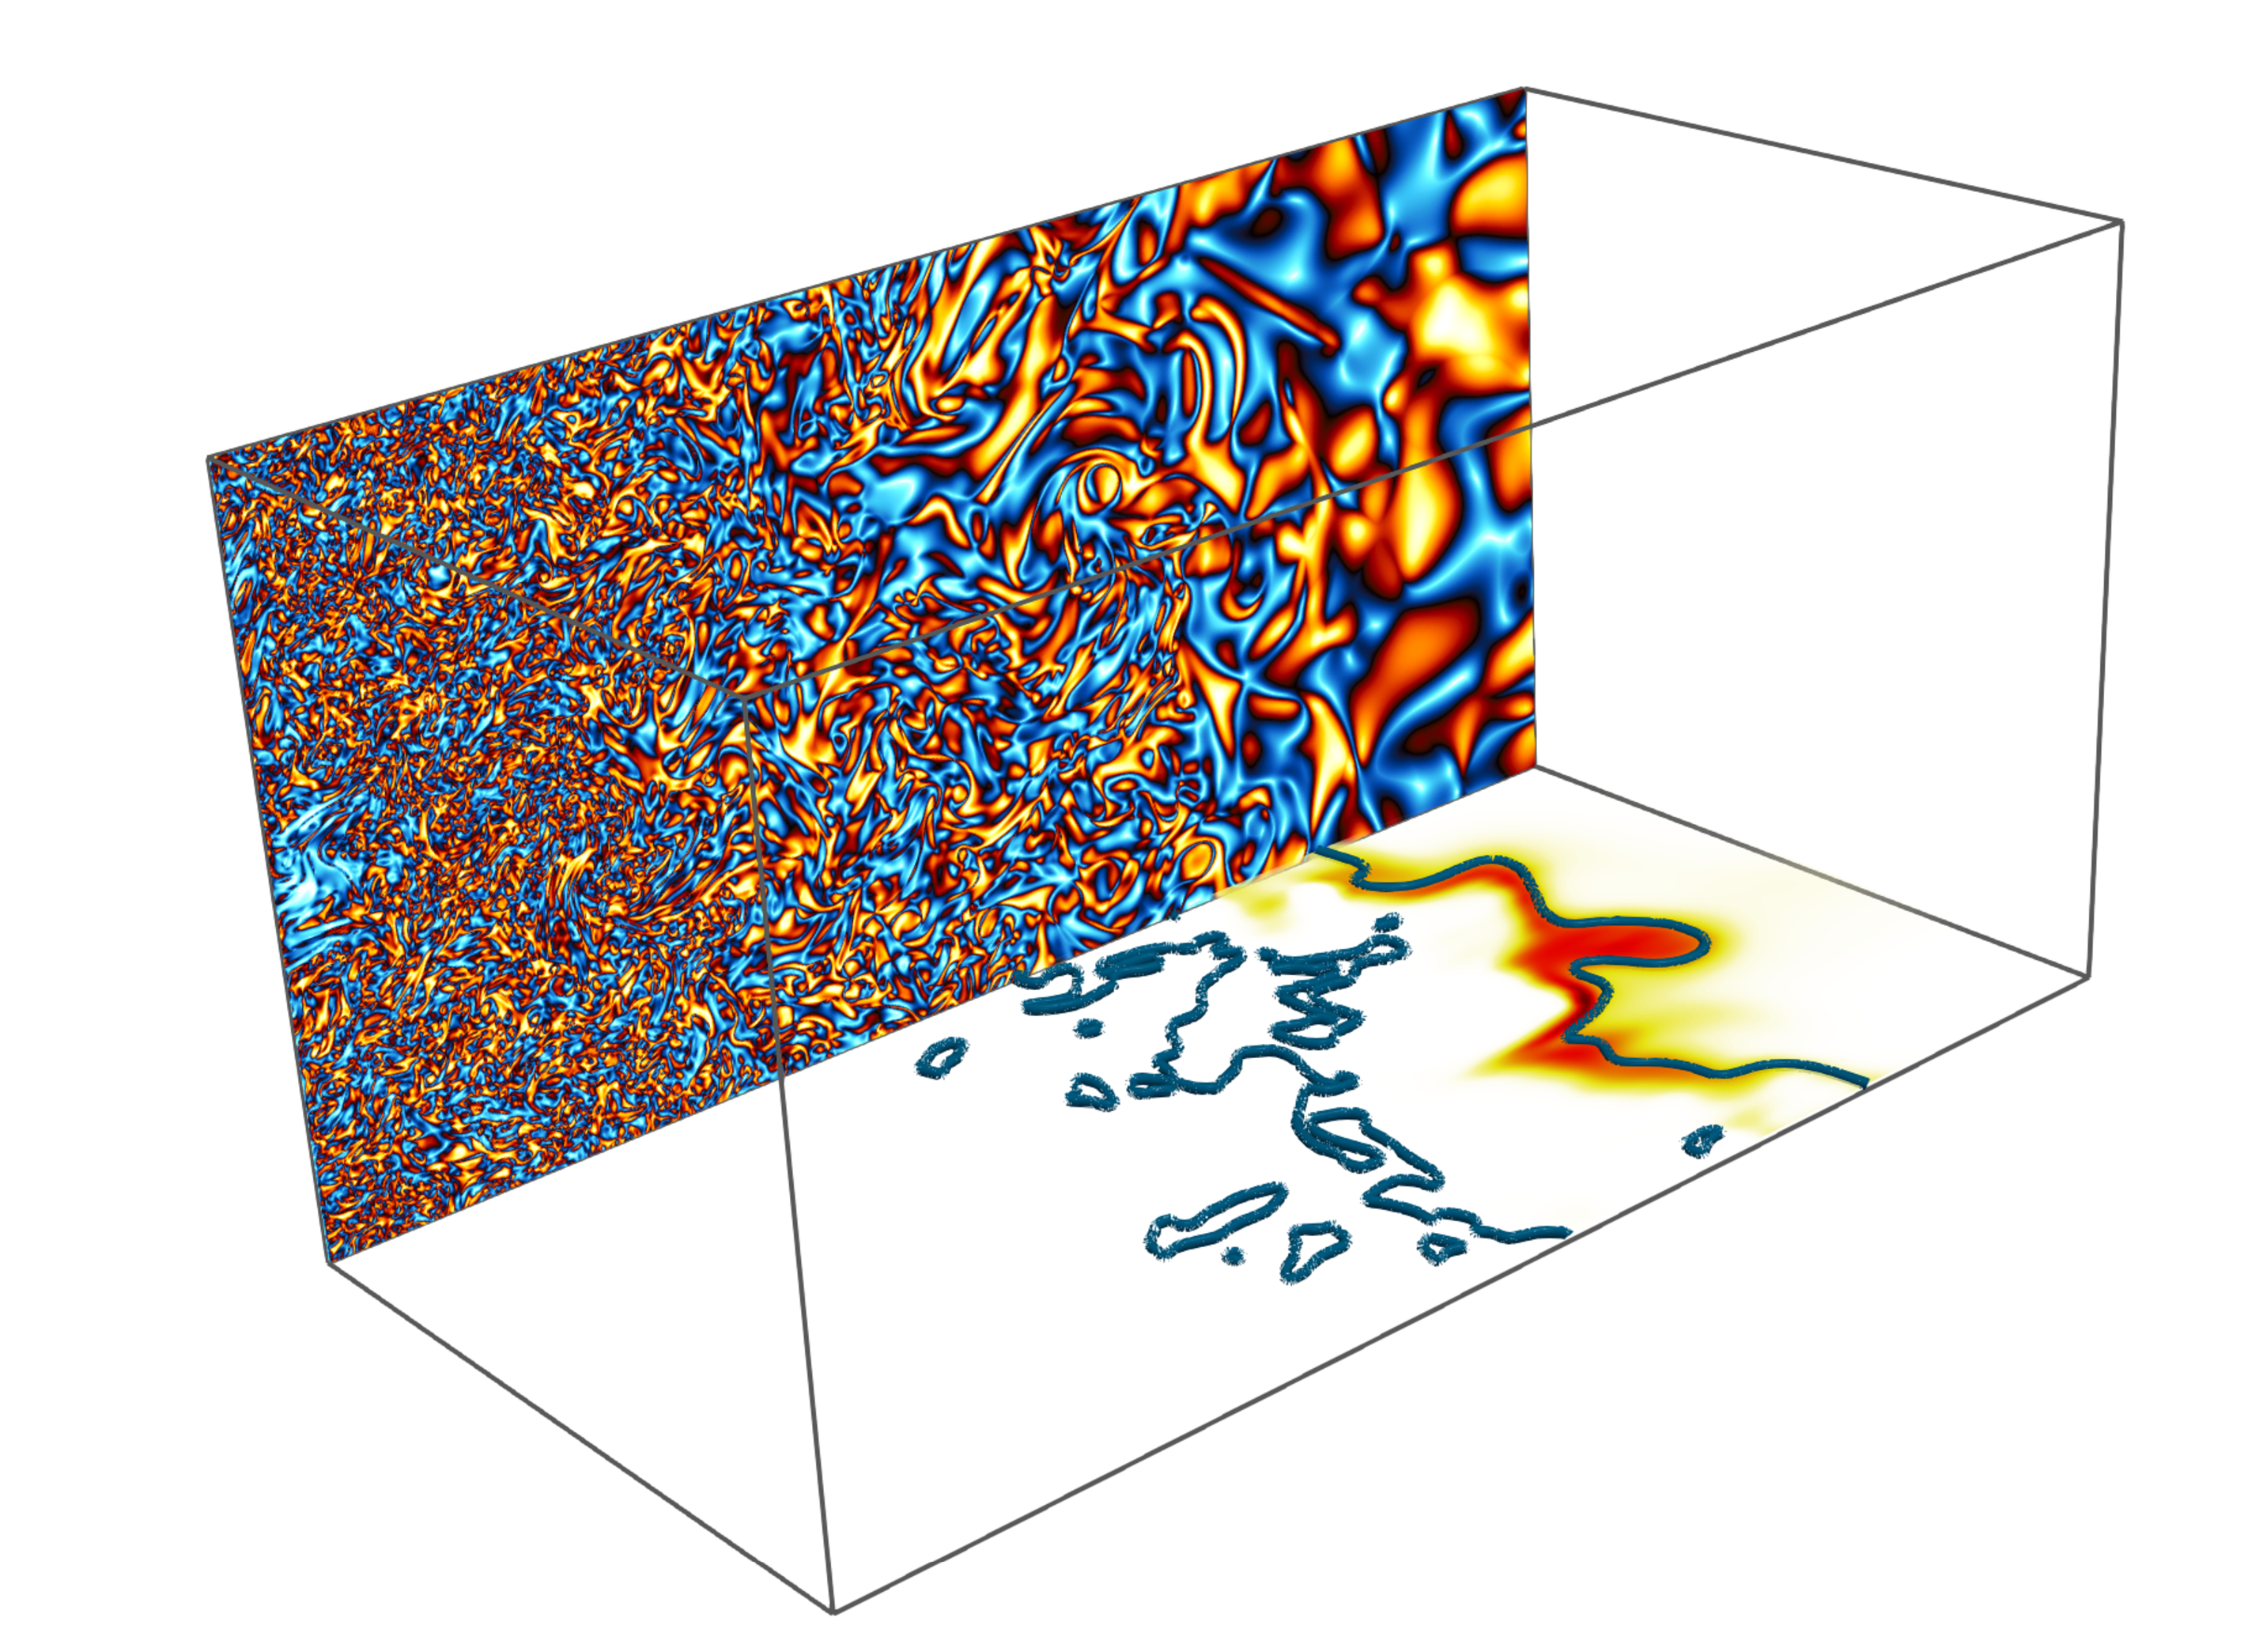
\includegraphics[width=.99\textwidth]{./figs/kappa/case4.pdf}
\caption{Case $\mathcal{C}_4$}
\label{fig:kappa_contour_case4}
\end{subfigure}
\caption{Instantaneous standardized difference between normal and non-normal contributions, 
$\kappa_{\mathcal{A}_{\mathcal{L}}, \mathcal{A}_{\mathcal{N}}}$, and normalized heat release rate 
$\hat{\dot{\omega}}_{\mathrm{HRR}}$. For all the cases, the inlet is on the left and the iso-lines
of the progress variable correspond to the values $c^*=0.4$ and $c^*=0.9$, where $c$ is the progress
variable based on the mixture temperature.}
\label{fig:kappa_contour}
\end{figure}
%
\autoref{fig:kappa_contour} shows that there are spatially localized, high-amplitude fluctuations
in the $\kappa_{\mathcal{A}_{\mathcal{L}}, \mathcal{A}_{\mathcal{N}}}$ field.
%
However, the occurrence of high non-normality zones is generally lower in the products side
in a sense that these effects are \emph{suppressed} by the flame.
%
These suppression abruptly takes place at the vicinity of the iso-surface $c^{*}=0.4$, which can be
viewed as a separation between the preheat and reaction zones, and it is more pronounced in lower
turbulence intensity (see \autoref{fig:kappa_contour_case1} and \autoref{fig:kappa_contour_case2})
in comparison to higher Karlovitz cases ($\mathcal{C}_3$ and $\mathcal{C}_4$ in 
\autoref{fig:kappa_contour_case3} and \autoref{fig:kappa_contour_case4}).
%
\begin{figure}
\begin{subfigure}{.48\textwidth}
\centering
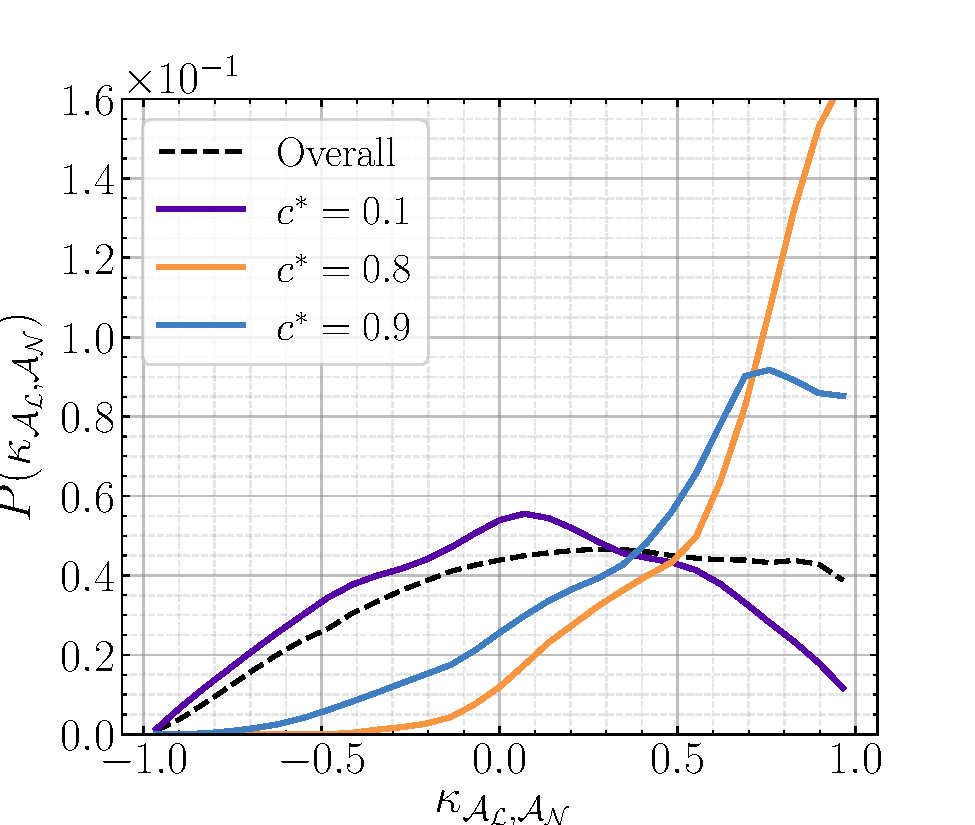
\includegraphics[width=.99\textwidth]{./figs/kappa_B_C_pdf/case1.pdf}
\caption{Case $\mathcal{C}_1$}
\label{fig:kappa_pdf_case1}
\end{subfigure}
%
\begin{subfigure}{.48\textwidth}
\centering
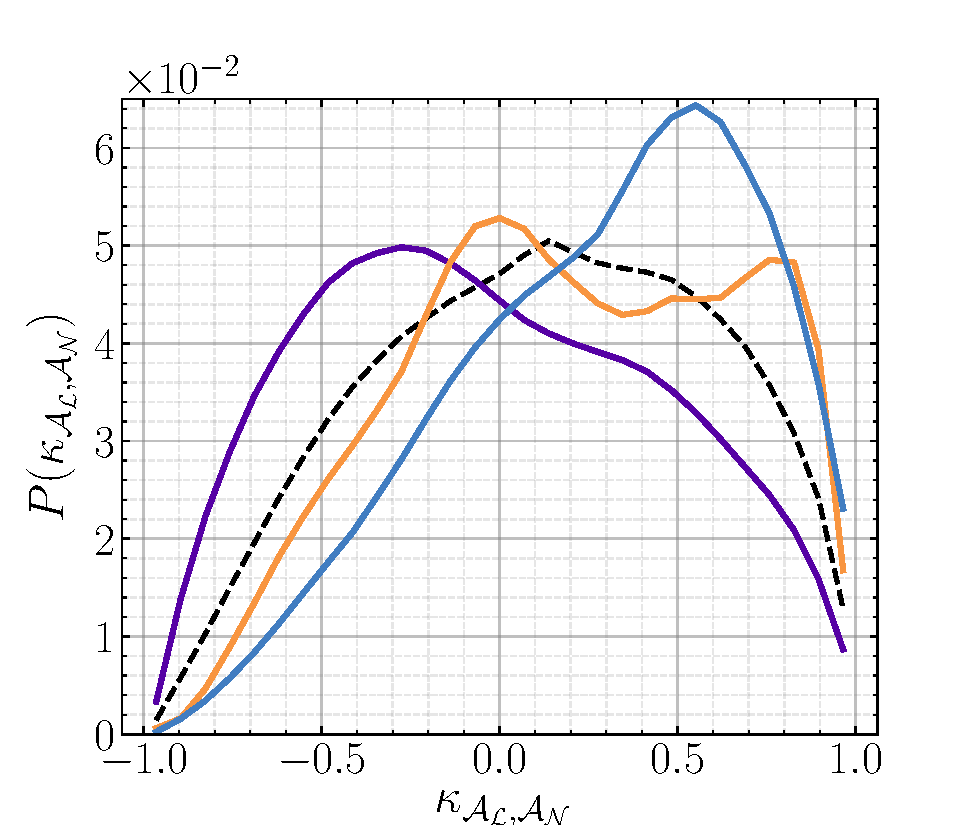
\includegraphics[width=.99\textwidth]{./figs/kappa_B_C_pdf/case2.pdf}
\caption{Case $\mathcal{C}_2$}
\label{fig:kappa_pdf_case2}
\end{subfigure}

\begin{subfigure}{.48\textwidth}
\centering
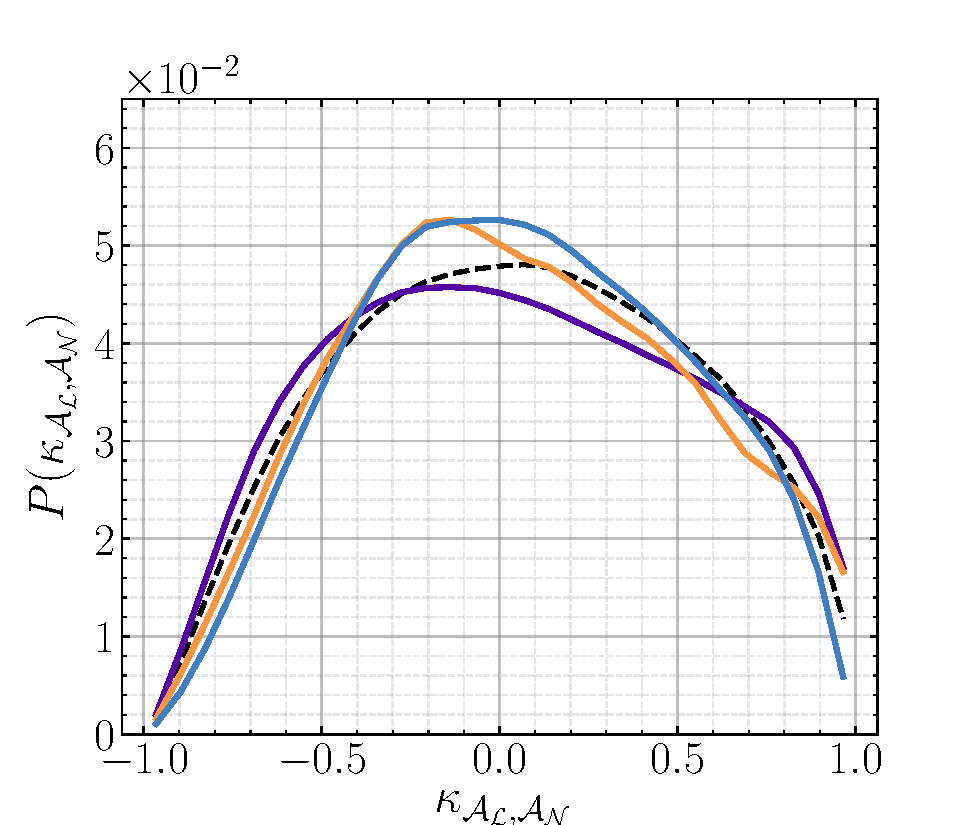
\includegraphics[width=.99\textwidth]{./figs/kappa_B_C_pdf/case3.pdf}
\caption{Case $\mathcal{C}_3$}
\label{fig:kappa_pdf_case3}
\end{subfigure}
%
\begin{subfigure}{.48\textwidth}
\centering
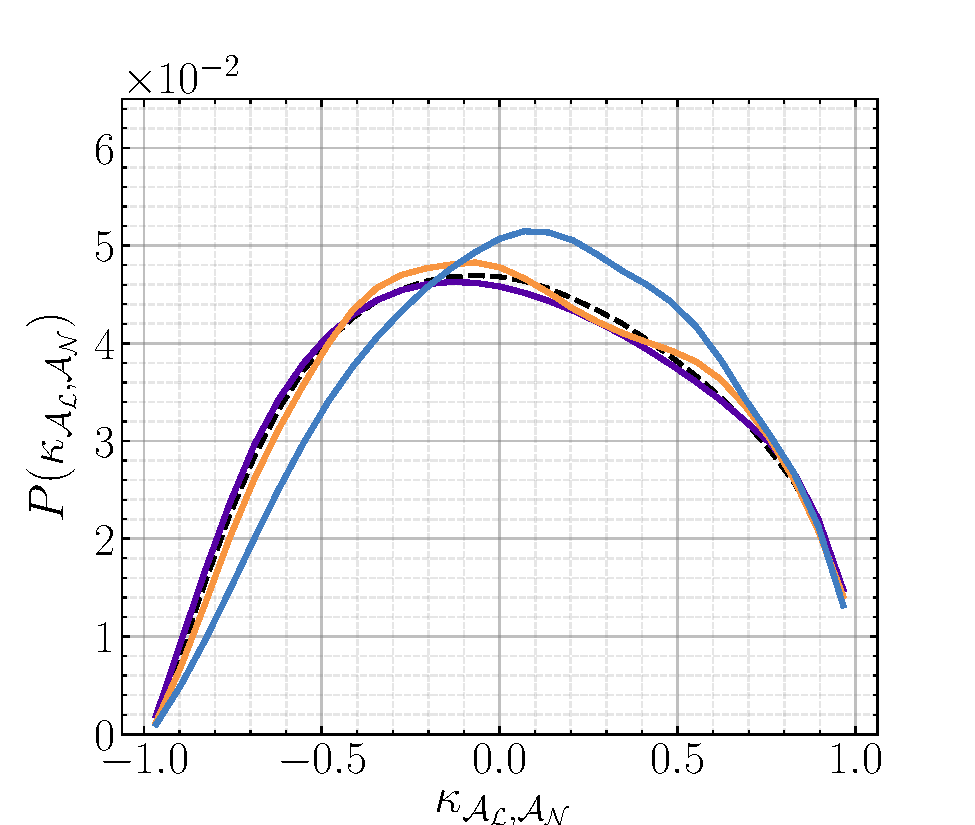
\includegraphics[width=.99\textwidth]{./figs/kappa_B_C_pdf/case4.pdf}
\caption{Case $\mathcal{C}_4$}
\label{fig:kappa_pdf_case4}
\end{subfigure}
\caption{Conditional PDF of the standardized difference between normal and non-normal contributions, 
$\kappa_{\mathcal{A}_{\mathcal{L}}, \mathcal{A}_{\mathcal{N}}}$. PDFs are shown for the iso-c values
0.1, 0.8 and 0.9, and the dashed line corresponds to the overall distribution. The values in parentheses
indicate the mode of the corresponding PDF.}
\label{fig:kappa_pdf}
\end{figure}
%%%%%%%%%%%%%%%%%%%%%%%%
% \hrule
%

% \begin{equation}
% a_N  = \mathbf{n}^{T}\boldsymbol{\mathcal{S}}\mathbf{n}
% \end{equation}
% %
% \begin{equation}
% a_T  = (\mathcal{\boldsymbol{I}} - \mathbf{n}\mathbf{n}^T):\boldsymbol{\mathcal{S}}
% \end{equation}
% %
% \begin{equation}
% a_T + a_N = \nabla \cdot \mathbf{u}
% \end{equation}
%

% \section{Conclusion}
% \label{sec:conc}
%=============================================================
% %==================================================================================================
\section*{Acknowledgements}
%==================================================================================================
The research reported in this paper was funded by King Abdullah University of Science and Technology.
The authors are thankful for the computing resources of the Supercomputing Laboratory and the Extreme Computing Research Center at King Abdullah University of Science and Technology. 
%
% \scriptsize
%=============================================================
\bibliographystyle{plainnat}
\bibliography{main.bib}
%=============================================================
\end{document}

